\documentclass[11pt,a4paper]{article}
\usepackage{amsmath,amssymb,unicode-math,lmodern}
\defaultfontfeatures{Ligatures=TeX}
\setmainfont[BoldFont=texgyrepagella-bold.otf,ItalicFont=texgyrepagella-italic.otf,BoldItalicFont=texgyrepagella-bolditalic.otf]{texgyrepagella-regular.otf}
\setmonofont[BoldFont=lmmonolt10-bold.otf]{lmmono10-regular.otf}
\setmathfont{texgyrepagella-math.otf}
\usepackage[margin=25mm,headheight=14pt,headsep=7mm]{geometry}
\usepackage{mathtools,booktabs,longtable,array,graphicx,xcolor,fancyhdr,needspace}
\newcolumntype{P}[1]{>{\raggedright\arraybackslash}p{#1}}
\usepackage[colorlinks=true,linkcolor=blue!40!black,citecolor=blue!40!black,urlcolor=blue!40!black]{hyperref}
\pagestyle{fancy}\fancyhf{}\lhead{\small Compact temporal encodings}\rhead{\small Paper III: draft v0.1}\cfoot{\thepage}
\setlength{\parskip}{4pt}\setlength{\parindent}{1.2em}\setlength{\emergencystretch}{2em}\raggedbottom
\newtheorem{theorem}{Theorem}[section]
\newtheorem{proposition}[theorem]{Proposition}
\newtheorem{corollary}[theorem]{Corollary}
\newtheorem{definition}[theorem]{Definition}
\newtheorem{remark}[theorem]{Remark}
\newenvironment{proof}{\par\noindent\textit{Proof.}\ }{\hfill$\square$\par}
\AddToHook{env/theorem/before}{\Needspace{7\baselineskip}}
\AddToHook{env/proposition/before}{\Needspace{7\baselineskip}}
\AddToHook{cmd/subsection/before}{\Needspace{7\baselineskip}}
\AddToHook{cmd/section/before}{\Needspace{10\baselineskip}}
\newcommand{\R}{\mathbb R}\newcommand{\C}{\mathbb C}
\newcommand{\norm}[1]{\lVert#1\rVert}
\newcommand{\ii}{\mathrm i}\newcommand{\dd}{\,\mathrm d}
\newcommand{\sinc}{\operatorname{sinc}}\newcommand{\clip}{\operatorname{clip}}
\newcommand{\rint}{\operatorname{rint}}\newcommand{\diag}{\operatorname{diag}}
\newcommand{\E}{\mathcal E}\newcommand{\Mat}{\mathrm M}
\newcommand{\Tp}{\mathcal T}\newcommand{\Pair}{\mathcal P}
\newcommand{\Amap}{\mathcal A}\newcommand{\Bmap}{\mathcal B}
\newcommand{\etaosc}{\eta_{\rm osc}}\newcommand{\qbox}{Q_{b,H}}
\hypersetup{pdftitle={Compact Temporal Encodings: Fourier Equivalence, Retrieval Obstructions and Saturation Effects},pdfauthor={Hilmir Frimann Halldorsson},pdfsubject={Paper III; local manuscript draft v0.1}}
\begin{document}
\begin{center}
{\LARGE\bfseries Compact Temporal Encodings:\par Fourier Equivalence, Retrieval Obstructions\par and Saturation Effects\par}
\vspace{5mm}{\large Hilmir Fr\'imann Halld\'orsson}\par
\vspace{3mm}19 October 2026\quad Paper III\quad Draft v0.1
\end{center}
\begin{abstract}
We examine what a five-real temporal representation inherited from a conditional periodic carrier preserves, what it loses, and what changes under numerical saturation. Completed pulses of exactly one circuit duration have a mean and one residual harmonic. Their directional coefficients are invertibly equivalent to two ordinary port Fourier moments. We prove an isolated timing-domain criterion, an aligned majority formula and an exact collision that prevents universal latest-order retrieval from the lossless aggregate. Retained observation data expose noisy-tie false decisions; matched software measurements favor direct timestamps for the narrow descriptor-to-order task and establish no general speed advantage. Event-wise quantization defines a different nonlinear map. We derive its chronological integer compositions, a sufficient corner-dominance domain, twelve-pair entrance bounds, a restricted suffix regime and the independent Fourier quantizer's corner abstention. Exact collisions, short covered errors and prefix dependence remain. At one-eighth-period lag, a monotone all-grid proof shows that the fixed 12-bit map reverses every final label after a sufficient 67 pairs. Complete retained operation and perturbation outcomes delimit the successful subset. Numerical projection changes the quadratic account and is not physical dissipation. The results separate information equivalence, decoder behavior and nonlinear numerical effects without a capacity or production-readiness claim.
\end{abstract}
\tableofcontents
\clearpage
\section{Question, scope and conventions}\label{sec:scope}
The paired-gap construction of Paper I provides a geometric setting for asking how a source state could be observed around an offset transverse circle.~\cite{PaperI} Paper II distinguishes that geometry from two additional comparison assumptions: a shared periodic carrier C1 and a passive exterior reception law C6.~\cite{PaperII} The present paper asks a computational question about a particular residual representation derived from those assumptions. How much of the timing of completed inputs survives in a compact state? Does its directional imbalance identify one pair, a history aggregate, or the last pair? What does coordinatewise saturation change?

Hilmir Frímann Halldórsson's motivation was to connect the paired construction and its observer responses to an explicit, testable temporal encoding. The investigations summarized here developed that question into a restricted event interface with matched Fourier and timestamp comparisons.~\cite{Pilot,Mechanism} A small state is useful only relative to a specified input and output contract. Neither a toroidal picture nor a successful subset of trials establishes general memory capacity.

We distinguish three objects: the exact lossless residual of C1; its finite-precision software representation; and a new, repeatedly projected numerical state. The third ceases to obey the first object's dynamics and work identity. The term SRG in retained empirical labels denotes the directional-coordinate implementation, not the native Tri-Octagon kernel or an entire family of character or memory systems. No native kernel, character-identity rule or physical receiver was evaluated in these comparisons.

The source record consists of the completed-pulse pilot and subsequent clipping-mechanism investigation, together with their internal mathematical/software reviews.~\cite{Pilot,Review09,Mechanism,Review10} The aligned majority formula and the clarification that the Fourier endpoint is an abstention are retained reviewer deductions. The proofs below state their hypotheses explicitly. Numerical results are the retained frozen comparisons; manuscript preparation introduces no new experimental corpus, performance measurement or decoder design.

\begin{table}[ht]
\centering\small
\begin{tabular}{P{30mm}P{119mm}}\toprule
Symbol & Meaning and convention\\\midrule
$L,c,T=L/c$ & Circumference, carrier speed and circuit time; $T$ is not a coordinate transform.\\
$\chi=s/R$ & Angle along the actual carrier circle, $L=2\pi R$.\\
$\epsilon=L/32$ & Source-tent arclength half-width, distinct from a physical shell or tube width.\\
$h,\rho$ & Height and radius of exterior arrays, retained from Papers I--II; never integer codes.\\
$\tau=t/T,\ d$ & Dimensionless analysis time and onset, common origin $\tau=0$.\\
$D,\phi$ & Pulse duration and common onset-phase offset; baseline $D=1$, aligned $\phi=0$.\\
$A,j$ & Nonnegative real source strength in $F_0$ units and port $j\in\{U,L\}$.\\
$\mu,z_U,z_L$ & Static mean and complex port moments in $F_0/c$ units.\\
$u_+,u_-$ & Directional amplitudes in the same units and global origin.\\
$\Mat,\Tp$ & Local complex matrix and real five-coordinate transform, not the native macro readout.\\
$b,H,\Delta$ & Bit width, numerical half-range and step $\Delta=2H/2^b$.\\
$K,\lambda,\upsilon$ & $K=2^{b-1}$ and integer endpoints $\lambda=-K,\ \upsilon=K-1$.\\
$(r,i)$ & Integer real/imaginary codes in a block; $i$ here is not $\ii=\sqrt{-1}$.\\
$\ell,N,D_N$ & Pair label, pair count and aligned count imbalance; $D_N$ is not duration.\\\bottomrule
\end{tabular}
\caption{Conventions separate geometry, time, source strengths and numerical storage. Geometric shell widths are not a quantizer step.}
\label{tab:conventions}
\end{table}

\section{Completed pulses and a five-real closure}\label{sec:closure}
\subsection{Inherited law and normalization}
On the circle, C1 is
\begin{equation}\label{eq:C1}
 p_t+c r_s=b_U(s)f_U(t)+b_L(s)f_L(t),\qquad r_t+c p_s=0,
\end{equation}
with zero preparation and periodic boundary conditions. Each $b_j$ is a translated unit-integral tent of half-width $\epsilon=L/32$. The paired contact angles and profile factors are
\begin{equation}\label{eq:geometry}
 \theta=\arctan(2/\sqrt3),\quad
 \chi_U=\pi-\theta,\quad\chi_L=\pi+\theta,\quad
 B_n=\sinc^2(n\pi/32),\quad \sinc x=\frac{\sin x}{x}.
\end{equation}
The circle, contact angle and exterior arrays are unchanged. Time normalization does not replace them by a unit-radius torus. Write $\widetilde p=cp/F_0$, $\widetilde r=cr/F_0$. An event is $f_j(t)=F_0 A h(\tau-d)$, where
\[
 h(q)=\sin^2(\pi q)\mathbf1_{[0,1]}(q),\qquad A\ge0 .
\]
It completes at $\tau=d+1$. Finite superpositions may overlap in time; closure is asserted only after all events have completed.

\begin{proposition}[Temporal moments and phase origin]\label{prop:moments}
For the positive temporal-transform convention, let
$I_n(d,A)=A\int_d^{d+1}h(\tau-d)e^{2\pi\ii n\tau}\dd\tau$.
Then $I_0=A/2$, $I_1=-Ae^{2\pi\ii d}/4$, $I_{-1}=\overline{I_1}$ and $I_n=0$ for integer $|n|\ge2$. A completed event adds
\begin{equation}\label{eq:event}
 z_e=-\frac{B_1A}{4}e^{-2\pi\ii d},\qquad
 \delta\mu=\frac A2,\qquad
 \delta u_\sigma=e^{\sigma\ii\chi_j}z_e,\quad \sigma=\pm1,
\end{equation}
with $u_\sigma$ referred to global normalized time zero.
\end{proposition}
\begin{proof}
Translate by $d$ and expand $h(q)=1/2-(e^{2\pi\ii q}+e^{-2\pi\ii q})/4$ on $[0,1]$. Orthogonality of integer exponentials gives the moments, including the negative sign. For an explicit sign check, the normalized characteristic field $(\widetilde p+\sigma\widetilde r)/2$ solves transport with source $LA b_jh/2$. Its spatial coefficient for $e^{-\sigma\ii\chi}$ is forced by $AB_1e^{\sigma\ii\chi_j}h/2$. The free factor is $e^{2\pi\ii\tau}$, hence variation of constants gives coefficient
$AB_1e^{\sigma\ii\chi_j}e^{2\pi\ii\tau}\int h(q-d)e^{-2\pi\ii q}\dd q/2$.
In the real-part convention that coefficient is $u_\sigma/2$, proving \eqref{eq:event} with the conjugate positive-time moment. The zero mode is $A/2$ since $T/L=1/c$ before normalization. The mean of $r$ remains zero by integrating its spatial derivative equation.
\end{proof}
A coefficient referred to $\tau_{\rm ref}$ multiplies $e^{2\pi\ii(\tau-\tau_{\rm ref})}$, so
\begin{equation}\label{eq:phase}
 u_\sigma^{(\tau_{\rm ref})}=e^{2\pi\ii\tau_{\rm ref}}u_\sigma^{(0)}.
\end{equation}
Paper II's one-period reference leaves it unchanged; its $3T/2$ reference multiplies it by $e^{3\pi\ii}=-1$. This conversion is common to both channels and every class. Reusing the latter coefficient at origin zero without this sign changes the waveform.

\begin{theorem}[Exact finite-family residual]\label{thm:closure}
For a finite superposition of completed events of the stated shape and duration, zero preparation and fixed contacts, define
\[
x=(\mu,\operatorname{Re}u_+,\operatorname{Im}u_+,\operatorname{Re}u_-,\operatorname{Im}u_-)\in\R^5
\]
by summing \eqref{eq:event}. After the last completion,
\begin{equation}\label{eq:residual}
 \begin{aligned}
 \widetilde p(\chi,\tau)&=\mu+\operatorname{Re}
 [(u_+e^{-\ii\chi}+u_-e^{\ii\chi})e^{2\pi\ii\tau}],\\
 \widetilde r(\chi,\tau)&=\operatorname{Re}
 [(u_+e^{-\ii\chi}-u_-e^{\ii\chi})e^{2\pi\ii\tau}].
 \end{aligned}
\end{equation}
No residual positive spatial mode above one remains. The coefficients need no update while sources are off.
\end{theorem}
\begin{proof}
The Fourier/characteristic solution of C1 is linear in its source. Each full event has zero temporal moment at every integer $|n|\ge2$, so its corresponding free residual coefficients vanish, even though the source tent has higher modes during forcing. The zero and first moments give \eqref{eq:residual}; finite superposition preserves it. The explicit free phase carries all subsequent motion. The stored amplitudes are therefore constant after completion. This proves the stated family closure, not a general forcing or active-event closure.
\end{proof}

\subsection{The interface is part of the claim}
A descriptor contains port, finite nonnegative onset, nonnegative amplitude and duration exactly one. It arrives at or after completion, in nondecreasing completion order. Zero amplitude changes neither coefficients nor timestamp validity; completion metadata may advance. A query requires a finite time at least the last completion and an explicit quiescent-batch promise. Five coordinates cannot detect an unseen active pulse. The implementation's unguarded algebraic \texttt{residual()} conversion is distinct from its guarded complete-state query.

Signal objects contain no raw history, pair ID, truth label, saved prior-state sequence or pending queue. The evaluator retains sorting, inputs and traces outside the encoder. Reset is explicit for independent pair trials; streams have no internal reset, subtraction, forgetting or normalization. Simultaneous descriptors supply no exact additive order feature. Nonlinear processing-order effects are separate and cannot manufacture temporal truth.

The timestamp comparator retains two last nonzero onsets, two validity flags and completion metadata. Nonoverlapping paired frames make these the final pair without pair IDs. It answers order and does not reconstruct fields. Raw-waveform acquisition and onset detection are outside all descriptor-input implementations.
\begin{figure}[ht]
\centering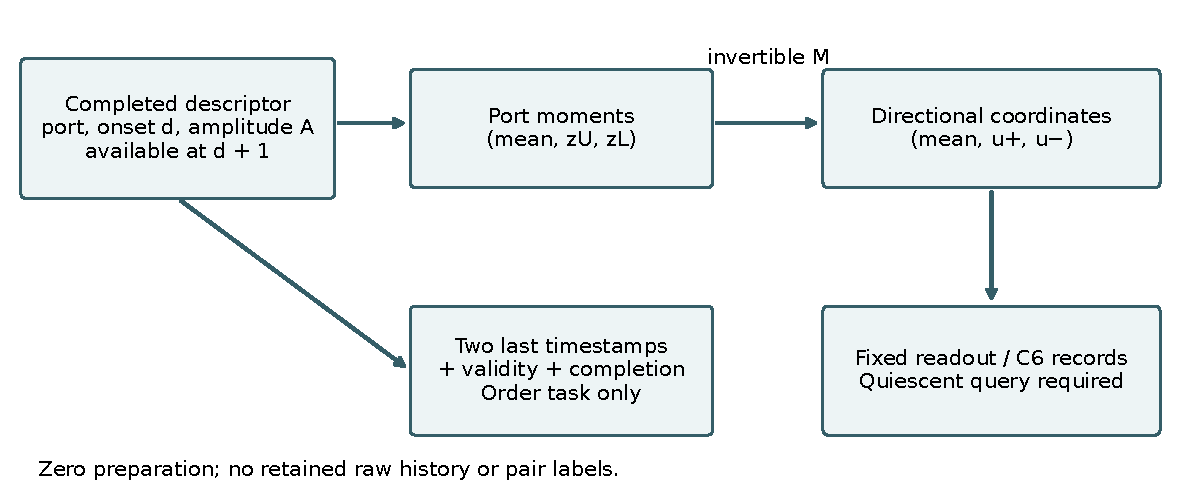
\includegraphics[width=\linewidth]{figures/fig01_interface.pdf}
\caption{Completed-event contract and exact basis equivalence. Arrows describe data access and algebra, not propagation in space. Completion and quiescence are required before exposing the residual.}
\label{fig:interface}
\end{figure}

\subsection{Storage, cross terms and the duration boundary}
The inherited normalized account and harmonic fraction are
\begin{equation}\label{eq:storage}
 \E(x)=\tfrac12\mu^2+\tfrac12|u_+|^2+\tfrac12|u_-|^2,\qquad
 \etaosc=\frac{|u_+|^2-|u_-|^2}{|u_+|^2+|u_-|^2}.
\end{equation}
The dimensional storage scale is $F_0^2L/c^2$. A zero harmonic denominator makes $\etaosc$ undefined. The total-storage fraction divides $(|u_+|^2-|u_-|^2)/2$ by $\E$, and is generally smaller in magnitude. For an additive increment $v$, expanding the square gives
\begin{equation}\label{eq:cross}
 \E(x+v)-\E(x)=x\cdot v+\tfrac12\norm v^2 .
\end{equation}
The account of a stream is not a sum of independent isolated-write accounts. C1's signed source-work law is conditional model mathematics, not native physical energy.

\begin{proposition}[Duration boundary and discarded tail]\label{prop:duration}
For $h_D(q)=\sin^2(\pi q/D)\mathbf1_{[0,D]}(q)$, $D>0$, put
$E(q,D)=(e^{2\pi\ii qD}-1)/(2\pi\ii q)$ for $q\ne0$ and $E(0,D)=D$. Then
\begin{equation}\label{eq:duration}
 I_n(D)=\tfrac12 E(n,D)-\tfrac14 E(n+D^{-1},D)-\tfrac14 E(n-D^{-1},D).
\end{equation}
For the retained two-unit-port stretched-pulse controls, the omitted normalized harmonic storage satisfies
\begin{equation}\label{eq:tail}
 \sum_{n>N}\E_n\le \frac{4\,32^4}{7\pi^6D^2N^7}.
\end{equation}
The omitted signed directional account has absolute value at most this bound.
\end{proposition}
\begin{proof}
Expansion of $\sin^2$ gives \eqref{eq:duration}, including the continuous zero-denominator values. Both $h_D$ and $h_D'$ vanish at the endpoints. Two integrations by parts give
$|I_n|\le(2\pi n)^{-2}\int_0^D|h_D''|\dd q$.
Here $h_D''=(2\pi^2/D^2)\cos(2\pi q/D)$, whose absolute integral is $4\pi/D$. Thus $|I_n|\le1/(\pi Dn^2)$. Each directional amplitude from two unit ports is bounded by $2B_n|I_n|$, regardless of onset/contact phases. Since $B_n\le32^2/(\pi^2n^2)$, its two-direction account is at most $4\,32^4/(\pi^6D^2n^8)$. Sum using $\sum_{n>N}n^{-8}\le\int_N^\infty x^{-8}\dd x=1/(7N^7)$. The absolute difference of nonnegative directional accounts is bounded by their sum.
\end{proof}
At $D=.98$ and $1.02$, the retained 70-digit evaluation through mode 512 gives discarded storage $5.24960914\,10^{-5}$ and $4.25775493\,10^{-5}$, with additional bounds $7.04\,10^{-17}$ and $6.50\,10^{-17}$. The first-mode projected fraction is $.989743319$ in both cases; full fractions are approximately $.989358003$ and $.989418686$. These are tail-qualified, non-interval decimal evaluations; the stated ratio reading allowance is $10^{-12}$, not a certified rounding enclosure. The primary API rejects both durations. Five coordinates then form only a projection, insufficient to synthesize the full carrier or exterior field.

\section{Fourier equivalence and exact information limits}\label{sec:equivalence}
\subsection{Independent implementations, equivalent information}
Let $y=(\mu,\operatorname{Re}z_U,\operatorname{Im}z_U,\operatorname{Re}z_L,\operatorname{Im}z_L)$, where $z_j$ sums the completed moments \eqref{eq:event} at port $j$. The moment implementation updates only that port. Its direct readout uses a cross product; conversion to directional coordinates is not imposed merely to make a comparison.

\begin{theorem}[Invertible coordinates and conditioning]\label{thm:transform}
The relation $x=\Tp y$ is induced by
\begin{equation}\label{eq:M}
 \begin{pmatrix}u_+\\u_-\end{pmatrix}
 =\Mat\begin{pmatrix}z_U\\z_L\end{pmatrix},\qquad
 \Mat=\begin{pmatrix}e^{\ii\chi_U}&e^{\ii\chi_L}\\
                         e^{-\ii\chi_U}&e^{-\ii\chi_L}\end{pmatrix}.
\end{equation}
Its determinant is $-8\ii\sqrt3/7$ and its singular values are $4/\sqrt7$ and $2\sqrt3/\sqrt7$. The harmonic condition number is $2/\sqrt3$. The real five-coordinate transform has singular values $1$, $4/\sqrt7$ twice and $2\sqrt3/\sqrt7$ twice, and condition number $4/\sqrt7$.
\end{theorem}
\begin{proof}
Write $C=\cos\theta=\sqrt{3/7}$, $S=\sin\theta=2/\sqrt7$. Then
\[
 \Mat=\begin{pmatrix}-C+\ii S&-C-\ii S\\-C-\ii S&-C+\ii S\end{pmatrix},
 \qquad\det\Mat=-4\ii CS=-8\ii\sqrt3/7 .
\]
The orthonormal symmetric/antisymmetric vectors diagonalize this normal matrix with eigenvalues $-2C$ and $2\ii S$. Singular values are their moduli. The interleaved harmonic real block is
\[
 \begin{pmatrix}
 -C&-S&-C&S\\ S&-C&-S&-C\\
 -C&S&-C&-S\\-S&-C&S&-C
 \end{pmatrix}.
\]
Realification repeats each complex singular value twice: a singular vector and its multiplication by $\ii$ span the corresponding real plane. The mean is an independent identity coordinate. Both harmonic singular values exceed one, so the full maximum/minimum ratio is $4/\sqrt7$. Nonzero determinant supplies the inverse.
\end{proof}
This exact information equivalence precedes nonlinear projection. Independent implementations can have different instruction counts; a change of basis does not create information or prove an algorithmic advantage.

\begin{proposition}[Direct moment readout]\label{prop:momentread}
With $w=z_U\overline{z_L}$, the numerator and denominator of $\etaosc$ are
\begin{equation}\label{eq:momentread}
 \begin{aligned}
 N_{\rm dir}&=4\sin(2\theta)\operatorname{Im}w,\\
 D_{\rm dir}&=2(|z_U|^2+|z_L|^2)+4\cos(2\theta)\operatorname{Re}w .
 \end{aligned}
\end{equation}
The denominator is positive for a nonzero pair of moments.
\end{proposition}
\begin{proof}
Expand both squared moduli in \eqref{eq:M}. Diagonal terms cancel in the difference and add in the sum. The two cross phases are $e^{-2\ii\theta}$ and $e^{2\ii\theta}$; their real-part difference is $2\sin(2\theta)\operatorname{Im}w$ and their sum is $2\cos(2\theta)\operatorname{Re}w$. The factor two from each modulus expansion gives the formulas. Positivity follows from $D_{\rm dir}=\norm{\Mat z}^2$ and invertibility.
\end{proof}

\subsection{Isolated order is periodic information}
\begin{theorem}[Isolated timing domain]\label{thm:isolated}
For one positive-amplitude completed pulse at each port, from zero preparation, $\operatorname{sign}\etaosc=\operatorname{sign}\sin(2\pi(d_L-d_U))$. This equals actual onset order for $0<|d_L-d_U|<1/2$. Simultaneity and half-period lags have zero numerator. Periodic aliases prevent extension to unrestricted onset differences.
\end{theorem}
\begin{proof}
Equation~\eqref{eq:event} gives
$z_U\overline{z_L}=B_1^2A_UA_Le^{2\pi\ii(d_L-d_U)}/16$.
The factor $4\sin2\theta$ and the denominator are positive. Sine has the required sign on $(-\pi,\pi)$, vanishes at integer multiples of $\pi$ and is periodic. For instance, positive lag $3/4$ gives a negative sine, while lag one gives zero. The restriction is mathematical, not a numerical defect.
\end{proof}
If one amplitude is zero, there are not two detected events whose order the feature can infer. The timestamp comparator uses the actual onset difference and its arithmetic tolerance; it is not restricted by phase periodicity.

\subsection{Aligned streams: majority, collision and mean growth}
A lower-late quarter pair, LQ or $\ell=+1$, places $U$ at $4m$ and $L$ at $4m+1/4$. UQ, $\ell=-1$, exchanges ports. All amplitudes are one and no reset occurs between pairs. Write $N_+,N_-$ for label counts, $N=N_++N_-$ and $D_N=N_+-N_-$.

\begin{theorem}[Aligned majority formula]\label{thm:majority}
Under these alignment, amplitude and quarter-lag hypotheses,
\begin{equation}\label{eq:majority}
 u_\pm=\frac{B_1}{4}(1-\ii)(NC\pm D_NS),\qquad
 \etaosc=\frac{4\sqrt3\,N D_N}{3N^2+4D_N^2}\quad(N>0).
\end{equation}
The feature gives the majority order, with a tie at $D_N=0$, and need not give the last order.
\end{theorem}
\begin{proof}
Put $c_0=B_1C/4$, $s_0=B_1S/4$. Substitution into \eqref{eq:event} gives LQ increment $(1-\ii)(c_0+s_0,c_0-s_0)$ and UQ exchanges its components. Integer-period translations leave them unchanged. Summing the two counts proves the first identity. Since $|1-\ii|^2=2$, the difference/sum of $(NC\pm D_NS)^2$ gives $2ND_NCS/(N^2C^2+D_N^2S^2)$, which reduces to the second. Its positive denominator leaves the sign of $D_N$.
\end{proof}

\begin{corollary}[Latest-order obstruction]\label{cor:collision}
The histories $[\mathrm{LQ}@0,\mathrm{UQ}@4]$ and $[\mathrm{UQ}@0,\mathrm{LQ}@4]$ have the same exact five-coordinate lossless state and last-completion metadata but different final labels. No deterministic decoder of those data can recover both final labels.
\end{corollary}
\begin{proof}
Both have $N=2,D_N=0$, $\mu=2$ and $u_+=u_-=B_1C(1-\ii)/2$. Their last completion is $4+1/4+1=21/4$. All allowed decoder inputs coincide, so its outputs coincide, while the required final labels are opposite.
\end{proof}
This is an obstruction for the commutative exact aggregate, not a theorem against all nonlinear encoders or an associative-memory capacity bound. Floating residues between theoretically identical histories are not robust stored labels.

Each pair adds one to $\mu$, so the mean account is $N^2/2$, equal to $8192$ at $N=128$. It is not $N$ independent slots. During the retained idle queries at extra delays $0,1,10^3,10^6$ periods the coefficients remained byte-identical. The maximum phase and output discrepancies were $1.99\,10^{-10}$ and $6.45\,10^{-10}$: effects of binary64 query-clock/argument reduction, not a million executed dynamical updates.

\begin{figure}[ht]
\centering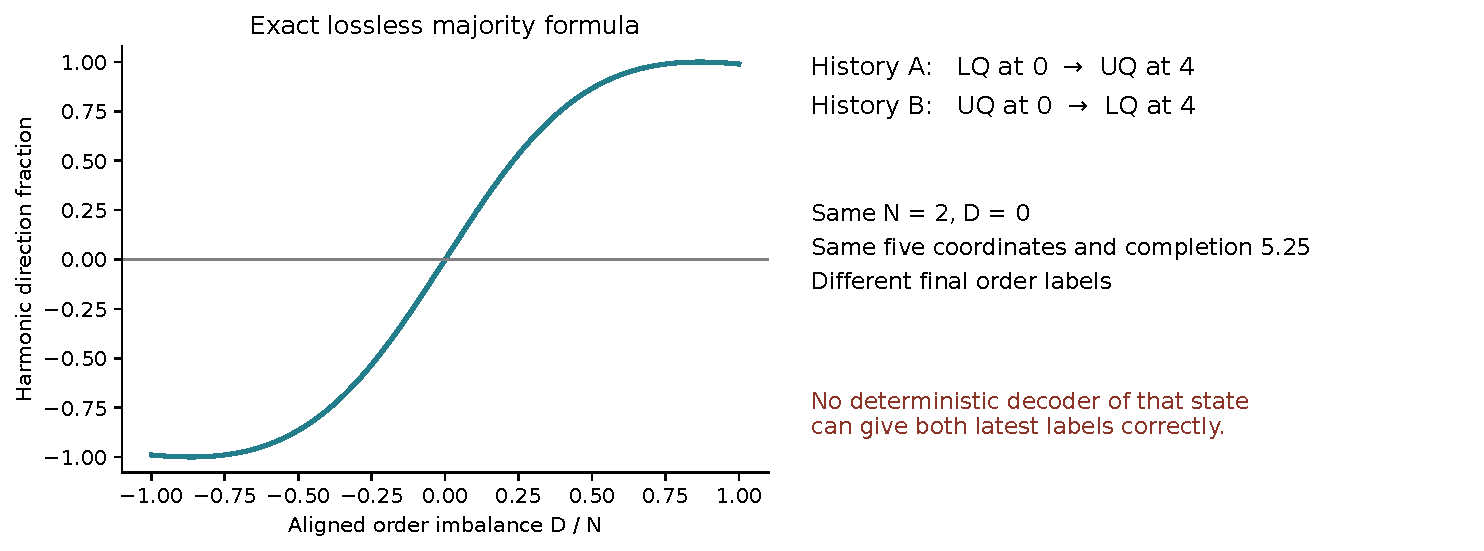
\includegraphics[width=\linewidth]{figures/fig02_aggregate.pdf}
\caption{Exact aligned aggregation. The curve illustrates the formula in $D_N/N$; finite counts occupy a discrete subset. The collision retains identical state and completion time but opposite final labels.}
\label{fig:aggregate}
\end{figure}

\section{Observation, precision and retained computational evidence}\label{sec:observations}
\subsection{The inherited observation map}
For a fixed exterior centre $X$, orthonormal frame $B_X$, tangent $\hat t(s)$ and distance $d_X(s)=\norm{X-\Gamma(s)}$, C6 adopts
\begin{equation}\label{eq:C6}
 \begin{aligned}
 U_X(t)&=\frac{g_o}{4\pi}\int_\Gamma\frac{p(s,t-d_X(s)/c_e)}{d_X(s)}\dd s,\\
 V_X(t)&=\frac{g_o}{4\pi}\int_\Gamma\frac{r(s,t-d_X(s)/c_e)\hat t(s)}{d_X(s)}\dd s,
 \qquad Y_X=(U_X,B_X^{\mathrm T}V_X).
 \end{aligned}
\end{equation}
This assumed straight-line delay and tangent-weighted reception does not feed back into C1. The centre-sampled observer geometry and all H/R arrays are those of Paper II. No new spoke, attachment or native coupling is inferred here. In normalized output units $g_oF_0/c$, the complete late residual record has the form
\begin{equation}\label{eq:record}
 Y(\tau)=D_o\mu+\operatorname{Re}\{Q u\,e^{2\pi\ii\tau}\},\qquad u=(u_+,u_-)^{\mathrm T}.
\end{equation}
For one site the two columns of $Q$ are
\[
 Q_\sigma=\frac1{4\pi}\int_\Gamma
 \frac{e^{-\sigma\ii\chi-\ii\beta d_X}}{d_X}
 \begin{pmatrix}1\\\sigma B_X^{\mathrm T}\hat t\end{pmatrix}\dd s,
 \quad \beta=\frac{c/R}{c_e}.
\]
The negative delay phase and signed vector column have different origins. $D_o$ is the mean-field reception vector. These matrices already include retarded spatial phase; synthesis adds no second delay.

Paper II proves complex rank two for a full off-circle site when $0\le\nu=c/c_e<\pi/2$, including $\nu=0,1$. Its circular symmetry reduction gives singular values $\sqrt{2(|H_o|^2+|S_o|^2)}$ and $\sqrt2|C_o|$ in unit gain, where $H_o,S_o,C_o$ are weighted cosine, sine-squared and cosine-squared moments. Equatorial scalar rows alone coincide in the directional columns: the odd sine integrand vanishes. Every equatorial scalar array is therefore rank one, even if many radii are present. A mirror pair off the equator or a calibrated full vector/scalar site can supply the missing complex direction. These are inherited rank statements, not new array optimization.

\begin{proposition}[Common phase/gain and sampled inversion]\label{prop:observation}
Suppose a known complex matrix $Q$ has rank two and samples are taken at $\tau_0+k/n$, $k=0,\ldots,n-1$, with $n\ge3$ and the usual DC, cosine and sine columns independent. In an exact first-harmonic record, fitting those columns gives phasor
\begin{equation}\label{eq:extraction}
 \widehat Y=(a_{\cos}-\ii a_{\sin})e^{-2\pi\ii\tau_0}.
\end{equation}
If all harmonic channels share an unknown factor $\gamma\ne0$, applying $Q^\dagger$ returns $\gamma u$, and $\etaosc$ is unchanged. The moment decoder may instead invert $Q\Mat$ and use \eqref{eq:momentread}.
\end{proposition}
\begin{proof}
For complex $h$, $\operatorname{Re}(he^{2\pi\ii k/n})=(\operatorname{Re}h)\cos(2\pi k/n)-(\operatorname{Im}h)\sin(2\pi k/n)$. At the common window origin $h=Q u e^{2\pi\ii\tau_0}$, proving the extraction sign and rotation. Full column rank gives $Q^\dagger Q=I$, hence $Q^\dagger(\gamma Q u)=\gamma u$. The common $|\gamma|^2$ cancels from the ratio. Invertibility of $\Mat$ proves the analogous moment statement. Independently unknown channel gains or clocks cannot generally be factored into one $\gamma$, so the conclusion does not extend to them.
\end{proof}
The retained interface uses eight equally spaced samples over one period with endpoint omitted. A clean 16-sample control is also retained. The window begins after the latest event end plus $D_{\max}/L$ for $\nu=1$. This accounts for retarded completion at every point. One known common window start is used in \eqref{eq:extraction}; no site-specific rephasing is fitted from truth. DC is retained even though the directional ratio ignores it. Observation-only decoders receive the same sample arrays, not event timestamps, noise realizations or hidden input labels.

\subsection{Numerical formats and uncertainty}
All event times, amplitudes and trigonometric evaluations are binary64; onset is reduced modulo one before phase evaluation. The float32 path casts each event increment before float32 accumulation. Its readout uses binary64 arithmetic and the declared band $|\eta|\le64\epsilon_{\rm state}$. This is mixed precision, not an all-float32 device. Samples stored as float32 are promoted for fitting and inversion, with a measurement-format band. The 8-,12-,16-bit coefficient formats are binary64 emulations of grid storage, not integer hardware.

The timestamp tolerance is $64\epsilon_{64}\max(1,|d_U|,|d_L|)$; time is not clipped to the coefficient range. Missing ports, invalid or nonpositive harmonic denominators and band-resolved ties return unresolved. A rank-one equatorial map always returns unresolved rather than guessing a direction.

The retained matrix qualifications separate quadrature/discretization, serialization and arithmetic. Entry allowances from the accepted reception data propagate to a group Frobenius bound; stacking uses the root sum of squares. The serialization contribution for an eight-entry complex full-site matrix is $\sqrt8\,10^{-14}$, with a $10^{-45}$ arithmetic term and the inherited analytic discretization allowance. These are non-interval numerical qualifications. An inverse error is amplified by its operator norm; the uniform eight-sample harmonic extraction has noise norm factor $\sqrt{2/8}$. For the retained groups the smaller singular value is about $.058430$ for the full site and $.019205$ for the mirror scalar pair (larger values $.107228$ and $.106241$). This explains a possible sensitivity difference without certifying a probability of success.

\subsection{Timing and noise outcomes}
The frozen isolated timing corpus has 7,680 unique perturbed pairs: 7,510 are in the sub-half-period domain and 170 are outside it; 150 actual orders reverse their nominal label, and no input-time quantization collision was recorded. Both coordinate implementations in each floating format correctly classify all 7,510 in-domain pairs. All 170 aliases are covered wrong decisions, as the sine criterion predicts. Timestamps correctly classify all 7,680. Counting actual rather than nominal order is essential.

The fixed-point isolated subset has 3,840 trials per width and basis. At eight bits the directional implementation gives 3,839 correct and one abstention; Fourier gives 3,838 correct and two abstentions. Widths 12 and 16 give 3,840 correct in both bases. No isolated trial saturated. Against the retained high-precision references, maximum first-timing-state errors were $3.61\,10^{-16}$ for float64 and $2.53\,10^{-8}$ for float32; matched observation coefficient comparisons were below $6.3\,10^{-16}$. These check implementation arithmetic, not C6 as a physical law.

Table~\ref{tab:noiseanchor} and Appendix~\ref{app:data} preserve all noise cells. For non-tie quarter controls there are 768 records per format/group/noise level; simultaneous controls have 384. At $\sigma=.01$, the full binary64 site is correct on 762/768 and the mirror scalar pair on 690/768; at $.1$, those counts are 490 and 419. Non-null quarter-control coverage is full in these binary64 cells. The coordinate decoders have zero decision disagreements.

\begin{table}[ht]\centering
\begin{tabular}{rrrr}\toprule
$\sigma$ & Full correct / 768 & Mirror correct / 768 & False simultaneous signs / 384\\\midrule
0 & 768 & 768 & 0\\
$10^{-5}$ & 768 & 768 & 384\\
$10^{-3}$ & 768 & 768 & 384\\
$10^{-2}$ & 762 & 690 & 384\\
$10^{-1}$ & 490 & 419 & 384\\\bottomrule
\end{tabular}
\caption{Retained binary64 counts. The last column applies separately to each non-null group. Clean simultaneous controls abstain; every tested positive noise level yields a spurious direction for all 384.}
\label{tab:noiseanchor}
\end{table}
The arithmetic band is not a statistical rejection policy. Noisy simultaneous controls falsely resolve at every tested nonzero level in both binary64 non-null groups. Float32's larger band changes some counts but is still not noise-aware. Equatorial nulls always abstain. Finite high accuracy on separated quarter pairs does not make the decoder reliable at ties. No threshold tuning or repair is introduced here.

The frozen channel-relative mismatch moves the lower-late quarter fraction from $.9897433$ to $.9948407$ while retaining its sign; the paired controls retain their reported signs. This breaks the common-factor premise but does not force a failure in this finite example. Calibration was not recovered from hidden truth or adjusted to obtain a desired result.

\subsection{Matched jobs and actual resource accounting}\label{sec:cost}
Three comparisons have different required outputs. J1 receives two completed descriptors and returns order. J2 receives the same events and returns the same eight-sample observation record, either at one site or all 84 sites. J3 receives only the given sample window and returns direction. Timestamps participate in J1 only: they do not have an equivalent field output and do not receive events in J3.

Corrected binary64 median microseconds per job were:
\begin{center}
\begin{tabular}{lrrr}\toprule
Job & Directional & Fourier & Timestamps\\\midrule
J1 events to order &17.263&19.210&12.933\\
J2 one-site record&40.403&45.196&---\\
J2 all-site record&64.534&67.250&---\\
J3 full-site samples&14.532&16.677&---\\
J3 mirror samples&14.653&17.817&---\\\bottomrule
\end{tabular}
\end{center}
Each timing cell has seven raw repetitions. The J1 min--max intervals are $12.087$--$19.651$, $13.582$--$19.690$ and $10.154$--$14.646$ microseconds. They overlap. Timestamps have the lowest narrow-task median; modest differences between coordinate implementations do not establish significance, complexity separation, tail latency, hardware acceleration or quantum advantage. Float32 does not automatically accelerate scalar Python.

J1/J2 include allocation, reset, validation, phase calculation, updates and the required output. J2 includes residual conversion, a guarded state copy and synthesis. J3 includes extraction, common phase conversion, inverse and classification. Corpus generation, reference calculations, plotting and I/O are outside these matched jobs. Shared calibration for the actual four-group/two-basis setup took $3.235$ ms, including an all-array inverse not needed by synthesis-only J2. Isolated median reset costs were about $.268/.272/.392$ microseconds and allocations $2.096/2.103/.733$ for directional/Fourier/timestamps; external sorting, descriptor construction and clock addition were separately recorded near $.494$, $.676$ and $.122$ microseconds.

Five float64 coefficients use 40 numerical bytes, or 20 in float32, with a 72-byte Python object and 112 bytes of array header. Timestamps use 16 bytes of onsets and two validity bytes, with a 56-byte object and 224 bytes of array headers. A completion float costs 24 Python bytes; format references, shared small objects and diagnostic metadata are additional. Logical payload and this interpreter's allocation footprint are different quantities.

Shared $\Mat$ and its inverse each use 64 numerical bytes. Full-site $Q,D_o$ use 128/32 bytes, its inverse another 128, and 8/16 extraction matrices total 576 bytes per decoder instance. All-site $Q,D_o$ use 10,752/2,688 bytes, plus 10,752 for each retained inverse. Eight full-site samples use 256/128 bytes in float64/32; all-site samples use 21,504/10,752. Headers and temporaries are additional; aliases are not separately allocated matrices. The evaluator's full histories and truth are outside the encoder but remain real process memory.

Descriptor availability is one period after onset. A late observation adds up to $1.5703786363$ periods in the recorded all-site setup, followed by acquisition of a one-period window; the last endpoint-omitting sample is at $7/8$ period. These physical/model-time latencies are not CPU microseconds. No waveform event detector is assigned a fictitious zero cost.

\begin{figure}[ht]
\centering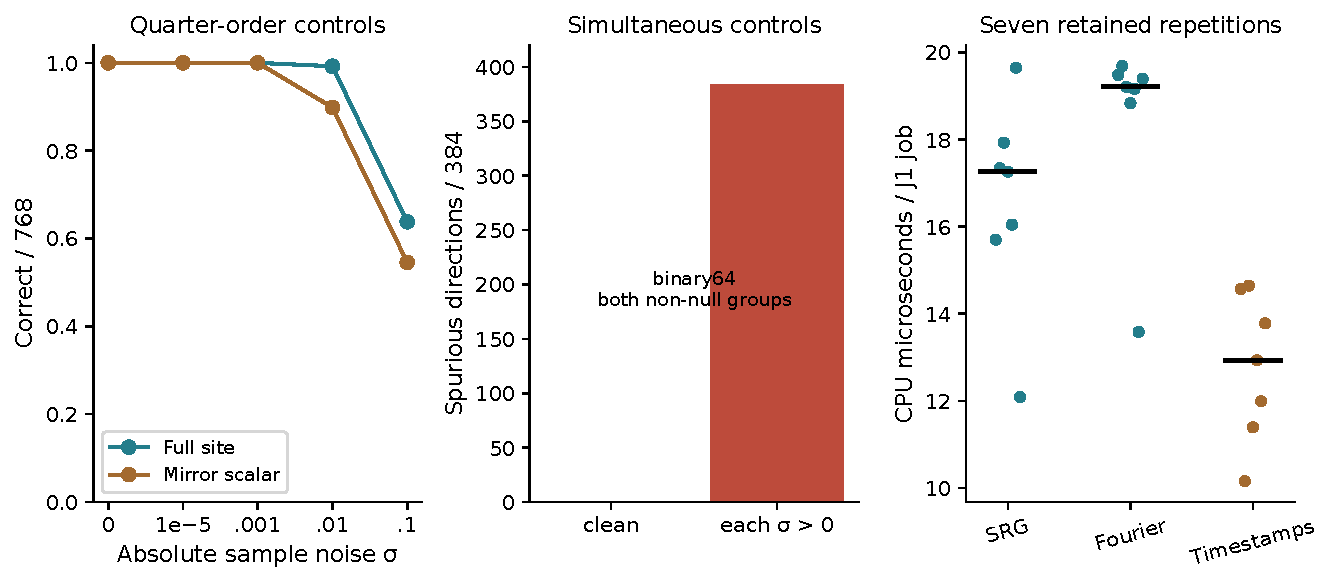
\includegraphics[width=\linewidth]{figures/fig03_measurements.pdf}
\caption{Retained corrected-run data: quarter-order noise accuracy, false simultaneous directions, and all seven J1 timing repetitions. Black timing marks are medians, not confidence intervals. Counts and time variability are distinct limits.}
\label{fig:measurements}
\end{figure}

\subsection{Two-run lineage and repeated-write evidence}
The pilot used Windows build 26200, an Intel64 Family 6 Model 183 Stepping 1 processor, 32 logical CPUs, Anaconda Python 3.11.15, NumPy 2.4.4 and QueryPerformanceCounter at reported 100 ns resolution. No CPU affinity, reserved host or hardware-energy counters were used. The first completed run took $51.44$ s with a reported 24-thread OpenBLAS configuration. Only a process configuration helper changed: it set thread variables before numerical imports, applied the existing pool limit and asserted the loaded thread count. The corrected run took $49.05$ s with one thread. The cause of the first launcher's missing variables was not established.

Both runs remain in the evidence. Three input corpora and eighteen saved data/summary files are byte-identical; timing, environment and elapsed metadata differ as expected. Only the corrected run supports the final timing claims. Per-directory no-rerun flags do not erase this two-run history. The original 178 checks, 26 result audits and later reviewer checks are inherited evidence, not newly executed manuscript tests.

At $N=128$, binary64 aligned alternating streams give zero coverage; aligned random orders give 54/96 correct with 89/96 covered. Random per-pair phases give 49/96 correct for alternating orders and 50/96 for random orders, with full coverage. Constant-label streams give 96/96 in either phase policy. These results agree with aggregation rather than universal recency.

The retained fixed-point subset is more striking: all 48 aligned random histories at length 128 are correct in directional coordinates at each width, while the Fourier path abstains on all 48. Every stream saturates; maximum coordinate-overflow counts are about 718--720 versus 477--479. The mean is below two instead of 128. The same histories are reused across widths, so these are not 144 independent successes. The next sections explain this distinct nonlinear effect and its failures.

\section{A different model: chronological quantization and saturation}\label{sec:maps}
\subsection{The event rule and exactness boundary}
The original finite-range operation, applied to each of the five coordinates after \emph{every event}, is
\begin{equation}\label{eq:quantizer}
 \qbox(v)=\Delta\,\clip\bigl(\rint(v/\Delta),-K,K-1\bigr),
 \qquad \Delta=\frac{2H}{2^b},\quad K=2^{b-1}.
\end{equation}
Here $\rint$ is nearest-integer rounding with ties to even, $H=2$ unless explicitly varied, and $b\in\{8,12,16\}$. Set $\lambda=-K$, $\upsilon=K-1$. The interval is asymmetric: $[-2,2-\Delta]$ in coefficient units. Its sign, range and fixed phase origin are retained.

For a quantized coordinate $\Delta k$ and unrounded event increment $v$, the ideal code update is
$k'=\clip(\rint(k+v/\Delta),\lambda,\upsilon)$.
Translation reduces this to a rounded integer addition only away from half ties. If $m-\tfrac12<v/\Delta<m+\tfrac12$, then adding integer $k$ places it strictly in the cell of $k+m$. At a tie the statement is false: $\rint(1+\tfrac12)=2$, whereas $1+\rint(\tfrac12)=1$. Floating addition can introduce an additional boundary qualification.

For the baseline constants
\begin{equation}\label{eq:cs}
 c_0=\frac{B_1}{4}\sqrt{3/7},\qquad
 s_0=\frac{B_1}{4}\sqrt{4/7},\qquad
 a=\rint(c_0/\Delta),\ b_0=\rint(s_0/\Delta),\
 p=a+b_0,\ d_0=b_0-a,
\end{equation}
the accepted rational certificates place every scaled constant strictly inside its stated rounding cell.~\cite{Mechanism} Table~\ref{tab:codes} records the consequences, with $w=\rint(B_1/(4\Delta))$.
\begin{table}[ht]\centering
\begin{tabular}{rrrrrrrrr}\toprule
$b$&$a$&$b_0$&$p$&$d_0$&$w$&$m_*$&$J$&$g$\\\midrule
8&10&12&22&2&16&12&6&253\\
12&167&193&360&26&255&12&7&101725\\
16&2673&3086&5759&413&4083&12&7&26830264\\\bottomrule
\end{tabular}
\caption{Certified baseline codes and derived bounds. $m_*$ is a sufficient same-label corner entrance count; $J$ bounds the restricted suffix family; $g=(K-1)^2-(K-d_0)^2$. These algorithmic counts have no inferred geometric meaning.}
\label{tab:codes}
\end{table}
Appendix~\ref{app:rational} states the rational enclosure construction and useful outward intervals. The source's 2,795,520 finite binary64 transition comparisons covered every incoming \emph{scalar} code for the admitted quarter-lag event types, coordinates, bases and widths. This exploits separability; it is neither a product-grid enumeration nor an all-platform transcendental proof. Our ideal-map statements use the certified mathematical codes. The large machine-grid checker is not rerun here.

\subsection{Deriving the actual pair maps}
The four harmonic event increments are obtained directly from \eqref{eq:event}:
\begin{equation}\label{eq:events}
\begin{array}{c|c|c}
\text{pair}&\text{early event}&\text{late event}\\\hline
\mathrm{LQ}&(c_0,-s_0,c_0,s_0)&(s_0,-c_0,-s_0,-c_0)\\
\mathrm{UQ}&(c_0,s_0,c_0,-s_0)&(-s_0,-c_0,s_0,-c_0).
\end{array}
\end{equation}
Each also adds $1/2$ to the mean. Completion order equals onset order for unit durations, so the late update is composed after the early update. Clipping the sum instead would change the algorithm.

\begin{theorem}[Chronological integer compositions]\label{thm:pairmaps}
On a harmonic code block $(r,i)\in[\lambda,\upsilon]^2$, define
\begin{equation}\label{eq:AB}
 \begin{aligned}
 \Amap(r,i)&=\bigl(\min(\upsilon,r+p),\ \max(\lambda,i-p)\bigr),\\
 \Bmap(r,i)&=\bigl(\max(\lambda,\min(\upsilon-b_0,r-d_0)),\
                         \min(\upsilon-a,i+d_0)\bigr).
 \end{aligned}
\end{equation}
For the certified codes, the event-wise LQ and UQ pair maps are
$\Pair_+=(\Amap,\Bmap)$ and $\Pair_-=(\Bmap,\Amap)$ on the plus/minus blocks. The mean code after a pair is $\min(\upsilon,k_\mu+2^{b-2})$.
\end{theorem}
\begin{proof}
Write $S_v(k)=\clip(k+v,\lambda,\upsilon)$. On the LQ active block the real updates are $+a,+b_0$ and the imaginary updates $-b_0,-a$. Positive increments compose as $S_{b_0}S_a(r)=\min(\upsilon,r+a+b_0)$; negative ones give the lower-saturating counterpart.

On its inactive block, real updates are $+a,-b_0$. Thus
$S_{-b_0}S_a(r)=\max(\lambda,\min(\upsilon,r+a)-b_0)
=\max(\lambda,\min(\upsilon-b_0,r-d_0))$.
Imaginary updates are $+b_0,-a$. Their composition is
$\max(\lambda,\min(\upsilon-a,i+d_0))$; the lower maximum is redundant since $i+d_0\ge\lambda$ and $\upsilon-a\ge\lambda$. This yields $\Bmap$. The UQ table exchanges active and inactive blocks. Each mean increment is exactly $(1/2)/\Delta=2^{b-3}$ code units; two positive increments give the displayed cap.
\end{proof}
The upper truncation $\upsilon-b_0$ in $\Bmap$ is an intermediate-event effect, not an arbitrary bound. At incoming real code $\upsilon$,
\[
 S_{-b_0}S_a(\upsilon)=\upsilon-b_0,\qquad
 S_aS_{-b_0}(\upsilon)=\upsilon-b_0+a .
\]
They differ. Repeated saturation destroys commutation and can retain an order-sensitive distinction that an additive sum loses.

\subsection{A sufficient corner mechanism}
Let $C_*=(\upsilon,\lambda)$ and $V=\norm{C_*}^2=(K-1)^2+K^2$.

\begin{theorem}[Incoming-state corner dominance]\label{thm:corner}
For any one of the three baseline widths, suppose the active incoming block of the final pair satisfies
\begin{equation}\label{eq:entry}
 r\ge\upsilon-p,\qquad i\le\lambda+p,
\end{equation}
and the other block is anywhere in the code square. Then the final active block is $C_*$ and the fixed directional readout has the correct sign. More precisely,
\begin{equation}\label{eq:margin}
 \ell\etaosc\ge\frac{g}{2V-g}>0,\qquad
 g=(K-1)^2-(K-d_0)^2 .
\end{equation}
\end{theorem}
\begin{proof}
The formula for $\Amap$ proves $C_*$ under \eqref{eq:entry}. Every $\Bmap$ output belongs to
$[\lambda,\upsilon-b_0]\times[\lambda+d_0,\upsilon-a]$.
For the listed constants $0<b_0<K$, so the real absolute value is at most $K$. Also $d_0>1$ and $d_0\le a+1$, so both imaginary endpoints have absolute value at most $K-d_0$. Thus $\norm{\Bmap}^2\le K^2+(K-d_0)^2=V-g$, and $g>0$. The label-signed ratio is $(V-q)/(V+q)$ for $q=\norm{\Bmap}^2\ge0$. This function decreases with $q$, giving \eqref{eq:margin}. All listed lower bounds lie well above the fixed arithmetic band.
\end{proof}
Every retained directional endpoint in the 48-history subset satisfies this sufficient active-corner condition at all three widths. That is a mechanism for the observed subset, not an assertion that every incoming history meets \eqref{eq:entry}.

\begin{proposition}[Twelve consecutive pairs and a restricted suffix regime]\label{prop:suffix}
From any harmonic code square, $m_*=\lceil(2K-1)/p\rceil=12$ consecutive identical baseline labels suffice to put their active block at $C_*$. Define
\begin{equation}\label{eq:Dk}
 D_k=\Bmap^k(C_*)=
 \left(\max(\lambda,\upsilon-b_0-(k-1)d_0),\
             \min(\upsilon-a,\lambda+kd_0)\right)\quad(k\ge1).
\end{equation}
For $1\le k\le J=1+\lfloor a/d_0\rfloor$ one has $\Amap(D_k)=C_*$. Here $J=6,7,7$. Consequently, states $(C_*,D_k)$ and $(D_k,C_*)$ have a conditional suffix description: repeating the current label increments $k$, while reversing the label resets to the exchanged state with $D_1$, provided every such use stays in $k\le J$.
\end{proposition}
\begin{proof}
Iteration gives $\Amap^m(r,i)=(\min(\upsilon,r+mp),\max(\lambda,i-mp))$. The maximum required coordinate travel across the square is $2K-1$, proving the sufficient count. For \eqref{eq:Dk}, the first inactive real step is $\upsilon-b_0$, then each step decreases by $d_0$ until the lower cap. The imaginary coordinate rises by $d_0$ until its upper cap. Induction proves the formula. The real entry requirement for $\Amap(D_k)$ is
$\upsilon-b_0-(k-1)d_0\ge\upsilon-p$, equivalently $(k-1)d_0\le a$.
The imaginary requirement follows from $kd_0\le a+d_0=b_0\le p$. For these widths the relevant values do not hit a cap that invalidates either inequality. Thus $\Amap(D_k)=C_*$. Now $\Amap(C_*)=C_*$ and $\Bmap(C_*)=D_1$; substitution into the two pair maps proves both conditional transitions.
\end{proof}
This does not assert entrance into the short-suffix family from every history. A long run can push its inactive block beyond the stated $J$ regime even though its active block remains at the corner. Twelve is a sufficient corner-entry count, not a minimal decision time, one-write replacement theorem or a count of physical openings.

\begin{figure}[ht]
\centering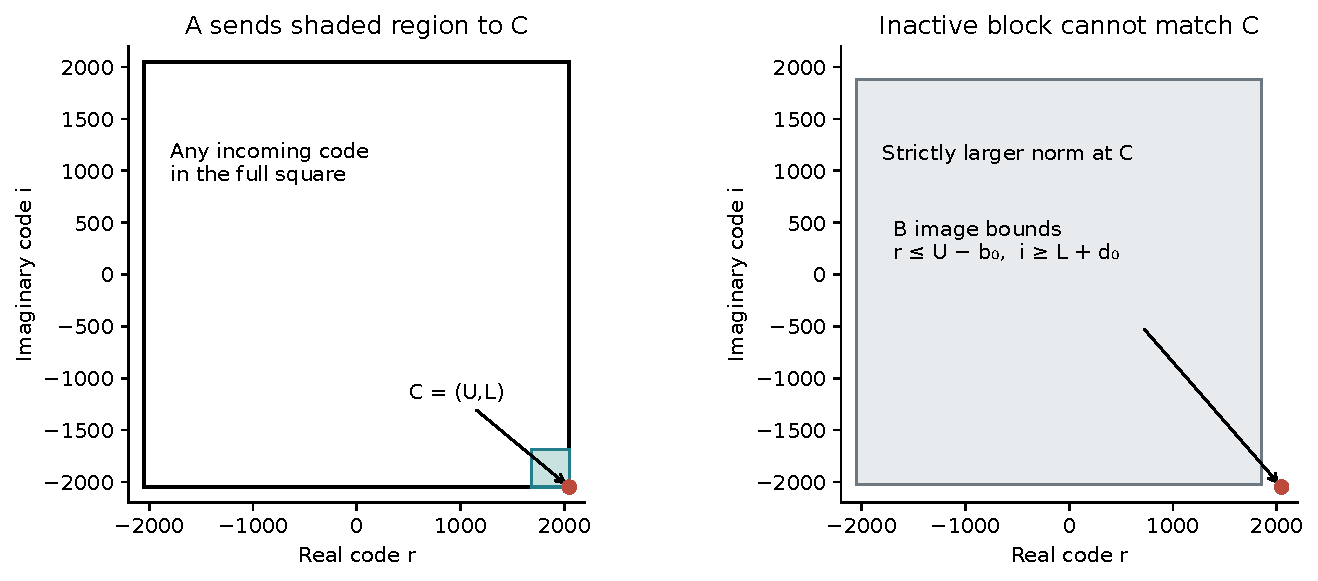
\includegraphics[width=\linewidth]{figures/fig04_corner.pdf}
\caption{Numerical code geometry at 12 bits; diagram labels $U=\upsilon$, $L=\lambda$, $C=C_*$. The final active map collapses its shaded incoming region to $C_*$. The inactive image has strictly smaller maximum norm. These rectangles depict numerical state space, not the toroidal construction.}
\label{fig:corner}
\end{figure}

\subsection{Independent Fourier clipping and same-operator conjugacy}
\begin{theorem}[Fourier corner abstention]\label{thm:fouriercorner}
For zero-start aligned quarter pairs under independent event-wise Fourier-axis quantization, let $n_+,n_-$ be the order counts. In code units,
\begin{equation}\label{eq:fouriercorner}
 \begin{aligned}
 z_U/\Delta&=-\min(K,n_+w)+\ii\min(\upsilon,n_-w),\\
 z_L/\Delta&=-\min(K,n_-w)+\ii\min(\upsilon,n_+w).
 \end{aligned}
\end{equation}
If both counts are at least $q_*=\max(\lceil K/w\rceil,\lceil\upsilon/w\rceil)$, equal to $8,9,9$ at the three widths, both moments equal $-K+\ii\upsilon$ in code units and the readout abstains.
\end{theorem}
\begin{proof}
An early aligned event adds the negative real moment $-B_1/4$, and a quarter-late event adds the positive imaginary moment $\ii B_1/4$. Port U is early on LQ and late on UQ, with the opposite assignments at L. Each affected coordinate therefore moves only one way, so repeated saturation is the capped count in \eqref{eq:fouriercorner}. The thresholds make both ports identical. Their cross product is real, so the numerator in \eqref{eq:momentread} is zero; the denominator remains positive by invertibility.
\end{proof}
All retained length-128 fixed-point histories meet both thresholds. Their complete state is $(\upsilon\Delta,(-K+\ii\upsilon)\Delta,(-K+\ii\upsilon)\Delta)$. Zero correct means 48 abstentions, not 48 reversed answers.

\begin{theorem}[Transporting the operator]\label{thm:conjugacy}
Let $Q$ be any fixed operation on the directional real state and $x=\Tp y$. If increments satisfy $v=\Tp w$, then the moment-coordinate operation
\begin{equation}\label{eq:conjugacy}
 y'=\Tp^{-1}Q\bigl(\Tp(y+w)\bigr)
\end{equation}
gives exactly $\Tp y'=Q(x+v)$. Applying the same axis-aligned coordinate quantizer independently to $y$ instead is generally a different nonlinear map.
\end{theorem}
\begin{proof}
Substitute $x=\Tp y$ and $v=\Tp w$, then multiply by $\Tp$. Since $\Tp$ is invertible, adjacent inverse factors cancel, proving equality at each event and by induction along every finite event list. Independent coordinate clipping would require $Q\Tp=\Tp Q$, which is false for a general mixing matrix: the inverse image of an axis box is an oblique cell set, not that same box.
\end{proof}
The saved conjugated control agrees after mapping back within $6.67\,10^{-16}$ at all 384 checkpoints, with identical decisions. Its transformed floating coordinates are not five independent $b$-bit Fourier values.

A common onset shift $\phi$ actively rotates both harmonic amplitudes by $e^{-2\pi\ii\phi}$. Lossless norms are invariant. A fixed asymmetric axis box is not generally rotation-covariant: even reversal of a boundary value can fall at the missing positive endpoint. A passive coordinate change $x'=Rx$ must transport increments, readout and box as $Q'=RQR^{-1}$. The frozen common-phase controls rotate the inputs relative to a fixed box; they are active tests, not passive relabellings or trial-specific rephasing.

\section{Exact failures and a uniform wrong-sign regime}\label{sec:failures}
\subsection{Collision, early covered error and prefix dependence}
The nonlinear map does not automatically eliminate the exact two-pair obstruction. Under the original quarter-lag round-and-clip rule, the histories $[-,+]$ and $[+,-]$ still collide at all three widths. To see this, after one positive pair the blocks are $(p,-p)$ and $(-d_0,d_0)$. The opposite pair sends both to $(p-d_0,-p+d_0)=(2a,-2a)$; the required intermediate values are inside their relevant caps for the listed widths. The reversed history exchanges equal blocks. At width 12 the full code state is
\begin{equation}\label{eq:clipcollision}
 (k_\mu,r_+,i_+,r_-,i_-)=(2047,334,-334,334,-334).
\end{equation}
Both abstain, their completion metadata agrees, and their final labels differ.

The earliest lexical \emph{covered} error in the retained binary-label tree is $[-,-,+]$, at starts $0,4,8$. Two negative pairs leave blocks $(-52,52)$ and $(720,-720)$ at width 12. Applying the final positive map gives
\begin{equation}\label{eq:three}
 (2047,308,-308,694,-694),\qquad
 \etaosc=\frac{308^2-694^2}{308^2+694^2}
       =-0.6708967909800521\ldots .
\end{equation}
Its last label is positive. The wrong negative answer is outside the band. Length one is correct, and the only opposite-label length-two histories are the collision; equal-label histories remain correct. Thus length three is the first possible covered error in this declared tree. The harmonic state here has not reached either corner.

Eight identical final labels also need not erase a prefix. Consider zero-start negative prefixes of lengths $n=32$ and $n=128$, followed by eight positive pairs. The negative prefix leaves the minus block at $C_*$ and the plus block at
\[
 \Bmap^n(0,0)=\bigl(\max(\lambda,-nd_0),\min(\upsilon-a,nd_0)\bigr).
\]
At width 12, the two terminal plus blocks are respectively $(2047,-2048)$ and $(832,-1000)$; the terminal minus block in both is $D_8=(1672,-1840)$. Hence
\begin{equation}\label{eq:eightsuffix}
 \eta_{32,+^8}=0.15126835330983474\ldots,\qquad
 \eta_{128,+^8}=-0.5701419258344036\ldots .
\end{equation}
These are exact integer-state calculations followed by a rational norm ratio. They have the same last eight labels and opposite predictions. They do not share identical absolute completion metadata, so this example establishes prefix dependence of the fixed harmonic readout, not the stronger equal-metadata collision claim of \eqref{eq:clipcollision}. Adding integer start shifts could align clocks without changing baseline phases, but no additional trial is needed for the stated prefix-dependence result.

The retained constant-prefix reversal controls test both initial signs, both bases, all three widths, prefix lengths 32/128 and opposite suffix lengths $1,2,4,8,16,32$. One-pair reversals fail in directional coordinates at every width. Suffix lengths 16 and 32 succeed for the directional controls, consistent with the sufficient twelve-pair entrance proof. Alternating-prefix controls are retained separately. No success at these lengths is promoted to a minimal overwrite bound.

\subsection{What a finite tree says about information}
The saved exhaustive tree contains all $2^1+\cdots+2^{12}=8190$ zero-start histories per width and basis, 49,140 endpoints in total. It is not the full four-coordinate code grid or all lengths. At depth 12, each directional width has 54 distinct states, with 2,972 correct and 1,124 covered wrong decisions among 4,096 histories, and no abstentions. There are no opposite-last-label collision states at that particular depth.

The Fourier tree at depth 12 has 13 states, 2,048 correct, 924 abstentions and 1,124 covered wrong decisions; 11 states have opposite last labels. Earlier directional collisions coexist with later finite label separation. The absence of a collision at one depth does not make the frozen norm-sign decoder correct there, nor establish arbitrary-length capacity. Conversely, a wrong decoder output is not by itself proof that the state contains no label information. No new decoder is fitted to the finite tree.

\subsection{One-eighth lag: exact endpoint and all-grid proof}
Change only the lag to $1/8$, keep amplitude one, aligned starts $4m$, width 12, $H=2$, the original asymmetric interval, fixed global origin and event-wise rounding/clipping. This lag is inside the isolated-pair timing domain. The failure below is not a half-period alias.

Let $c_0,s_0$ be as in \eqref{eq:cs}, and define
\[
 e=\frac{s_0-c_0}{\sqrt2}>0,\qquad
 f=\frac{s_0+c_0}{\sqrt2},\qquad
 e_0=\rint(e/\Delta)=18,\quad f_0=\rint(f/\Delta)=255.
\]
Their strict rounding cells are rationally certified. The equality $f_0=w=255$ is only an equality of rounded codes; $f$ and $B_1/4$ are not identical.

\begin{theorem}[All-grid finite-entry reversal]\label{thm:eighth}
Under precisely these ideal-map assumptions, from any incoming harmonic grid state and any incoming mean, every label sequence of length at least 67 has a final fixed-readout sign opposite to its final label. The two terminal harmonic signatures, in code units, are
\begin{equation}\label{eq:signature}
 \ell=+1:\quad(\upsilon,\lambda+e_0,\upsilon-e_0,\lambda),
 \qquad
 \ell=-1:\quad(\upsilon-e_0,\lambda,\upsilon,\lambda+e_0).
\end{equation}
For both,
\begin{equation}\label{eq:wrongmargin}
 \ell N_{\rm dir}=2e_0(\upsilon+\lambda)\Delta^2
       =-\frac9{262144},\qquad
 \ell\etaosc=-2.16577126062446\,10^{-6}\ldots .
\end{equation}
The bound 67 is sufficient, not claimed minimal.
\end{theorem}
\begin{proof}
For LQ the early event is the first row of \eqref{eq:events}. At phase $\pi/4$, the late L event has harmonic increment $(f,e,-e,-f)$. UQ's late U event has $(-e,-f,f,e)$, exchanging the eventual block roles. Non-half-cell translation therefore gives the following LQ block actions:
\begin{equation}\label{eq:eighthmaps}
 \begin{aligned}
 r_+'&=\min(\upsilon,r_++a+f_0),&
 i_+'&=\max(\lambda+e_0,i_+-(b_0-e_0)),\\
 r_-'&=\min(\upsilon-e_0,r_-+a-e_0),&
 i_-'&=\max(\lambda,\min(\upsilon-f_0,i_--(f_0-b_0))).
 \end{aligned}
\end{equation}
For example, the plus imaginary composition first subtracts $b_0$, clips below, then adds $e_0$; the upper clip is redundant because $b_0>e_0$. The minus real composition first adds $a$, then subtracts $e_0$; its lower clip is redundant because $a>e_0$. UQ exchanges these two block maps. Thus, under either label, each real code satisfies
\begin{equation}\label{eq:drift}
 r'\ge\min(\upsilon-e_0,r+149),\qquad
 i'\le\max(\lambda+e_0,i-62)
\end{equation}
for each imaginary code. Indeed $a-e_0=149$, $a+f_0=422\ge149$; $b_0-e_0=175\ge62=f_0-b_0$. The extra upper cap in the last line of \eqref{eq:eighthmaps} can only decrease its output, preserving the upper comparison.

Monotonicity allows iteration of these scalar comparisons for any sequence of labels. Starting with $r\ge\lambda$ gives
$r_n\ge\min(\upsilon-e_0,\lambda+149n)$.
Starting with $i\le\upsilon$ gives
$i_n\le\max(\lambda+e_0,\upsilon-62n)$.
The distance to the required boundaries is $2K-1-e_0=4077$; hence
\[
 n_r=\lceil4077/149\rceil=28,\qquad
 n_i=\lceil4077/62\rceil=66 .
\]
All four harmonic coordinates lie in
\begin{equation}\label{eq:rectangle}
 \mathcal R=\bigl([\upsilon-e_0,\upsilon]\times
                         [\lambda,\lambda+e_0]\bigr)^2
\end{equation}
after at most 66 pairs. The comparisons show that these lower/upper thresholds persist; the global code caps give the other two sides, so $\mathcal R$ is invariant.

Now take an incoming state in $\mathcal R$ and apply LQ. The plus real coordinate reaches $\upsilon$ since $a+f_0\ge e_0$; the minus real coordinate reaches $\upsilon-e_0$ since $a\ge e_0$. The plus imaginary coordinate reaches $\lambda+e_0$ since $b_0-e_0\ge e_0$. The minus imaginary coordinate reaches $\lambda$ since $f_0-b_0\ge e_0$. These are the literal inequalities $422\ge18$, $167\ge18$, $175\ge18$, $62\ge18$. Thus the next pair gives \eqref{eq:signature}; UQ exchanges the blocks. Both signatures lie in $\mathcal R$, so every subsequent pair again produces its own corresponding signature. This proves the arbitrary-label statement from pair 67 onward.

The label-signed squared-norm difference is
\[
 \upsilon^2+(\lambda+e_0)^2-(\upsilon-e_0)^2-\lambda^2
 =2e_0(\upsilon+\lambda)=-36 .
\]
Since $\Delta=1/1024$, this is $-9/262144$ in coefficient-squared units. The positive denominator is
\[
 [2047^2+(-2030)^2+2029^2+(-2048)^2]/1024^2
 =15.8522167205810546875 .
\]
Division gives \eqref{eq:wrongmargin}. Its magnitude is greater than $64\epsilon_{64}$, so the fixed rule resolves a strictly wrong sign rather than abstaining. The independent mean coordinate never enters this comparison.
\end{proof}
The retained 48 binary64 endpoints agree with these signatures. They are implementation instances, not a formal guarantee for every platform's arithmetic. The universal theorem rests on the ideal integer compositions and certified constants, not on the sampled histories or the earlier quarter-lag scalar-grid audit.

The two signatures are still label-dependent; the frozen energy-sign readout interprets them backwards. Reversing a sign for one known cell would be a new decoder design, not an information theorem or a universal repair. If one algebraically substitutes symmetric endpoints, the expression $2e_0(\upsilon+\lambda)$ becomes zero. That hypothetical combined eighth-lag/symmetric-endpoint control was not executed or adopted. No sign or endpoint is changed here.

\begin{figure}[ht]
\centering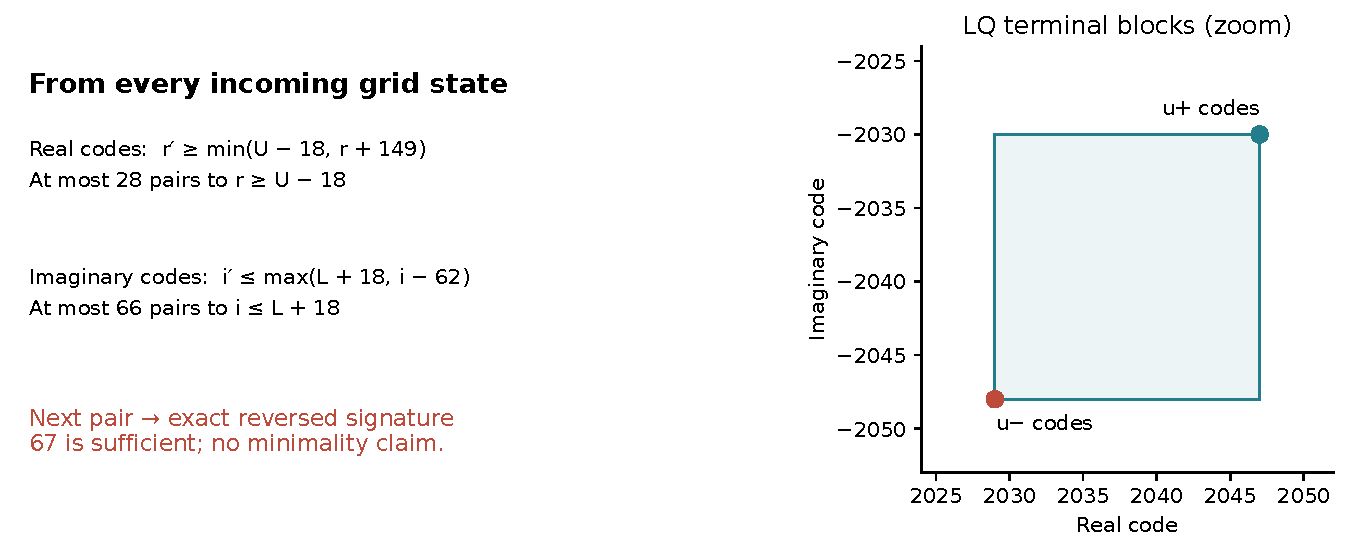
\includegraphics[width=\linewidth]{figures/fig05_eighth.pdf}
\caption{A sufficient all-grid proof, not a simulated convergence plot; $U=\upsilon$ and $L=\lambda$. Scalar comparisons put every block in the invariant rectangle by pair 66; the next pair creates the reversed signature. The zoom shows its two LQ blocks in numerical code space.}
\label{fig:eighth}
\end{figure}

\section{Operation controls, perturbations and the changed account}\label{sec:controls}
\subsection{What the operation comparison isolates}
The fixed operation study reuses exactly the same 48 aligned random-order histories of length 128, with width 12 and $H=2$. LOSSLESS performs no projection; ROUND\_ONLY rounds but has no finite code limit; CLIP\_ONLY continuously clips to $[-H,H-\Delta]$ without rounding. ROUND\_CLIP is \eqref{eq:quantizer}. SYMMETRIC\_ENDPOINT changes its code interval to $[-\upsilon,\upsilon]$, retaining the step but removing one code.

PAIR\_CLIP sums two events inside an evaluator-declared pair, then applies the original quantizer. It requires grouping/buffering unavailable to the primary autonomous event encoder and changes intermediate availability. FINAL\_CLIP projects the lossless sum once, at readout; its prefix snapshots do not feed back into future updates. CONJUGATED\_Q implements \eqref{eq:conjugacy}. These are mechanism controls, not equal-access online competitors or equal-bit-capacity implementations. Continuous values and unbounded integer codes must not be described as $b$-bit storage.

All fifteen basis/operation endpoints are in Appendix~\ref{app:data}. Directional LOSSLESS and ROUND\_ONLY both give 26 correct, three abstentions and 19 covered wrong answers out of 48. CLIP\_ONLY and ROUND\_CLIP give 48 correct, with minimum signed margins $.0539047886$ and $.0539720997$. The symmetric endpoint also gives 48 correct. Thus repeated saturation is responsible for this subset effect; rounding and endpoint asymmetry are not necessary for that particular positive quarter-lag result.

PAIR\_CLIP also gives 48 correct, with smaller minimum signed margin $.0127790302$, despite its different cadence. FINAL\_CLIP gives 48 abstentions. The independently clipped Fourier variants abstain on all 48 for every clipping operation. Fourier LOSSLESS and ROUND\_ONLY reproduce 26/3/19. CONJUGATED\_Q returns 48 correct and the same directional margins within the recorded arithmetic tolerance. These controls isolate the operator, not an advantage from renaming coordinates.

\subsection{All fixed perturbation classes}
The sixteen cells retain the same 48 order sequences. They change one factor at a time: common phases $1/16,1/8,1/4,3/8$; independent per-pair common phases; lag $1/8$ or $3/8$; common amplitudes $1/4$ or $2$; upper-only or lower-only amplitude reduction to $1/2$; bounded onset jitter; numerical range $H=1$ or $4$; or symmetric endpoints. The baseline is the remaining cell. Increasing $H$ at fixed bits also changes $\Delta$, so these are not range-only tests at fixed resolution.

The saved nuisance generator was PCG64 with SeedSequence parameters [old root,10,cell ID,old trial]; no new random orders were drawn. Jitter was uniform in $[-1/64,1/64]$, with U then L draws and a common integer offset two to keep onsets nonnegative. Actual order did not reverse in that cell. The current manuscript reads those outcomes; it does not regenerate draws.

Common phases preserve the directional signs for this subset but change margins and states. Independent pair phases give only 22/48 correct, all covered, versus Fourier 24/48. Lag $3/8$ yields directional 39 correct and nine wrong, Fourier 31 correct, one abstention and 16 wrong. Upper-half amplitude gives directional 45 correct/three wrong; lower-half gives 39/nine. The eighth-lag cell gives 48 covered wrong directional answers and 48 Fourier abstentions, as explained by Theorem~\ref{thm:eighth}. The jitter cell gives directional 48 correct and Fourier 41 correct/seven abstentions. The complete table includes the successful amplitude, range and endpoint cells; none removes the failed domains.

There are 768 perturbed histories and 12,288 reported basis/prefix records. Timestamps correctly identify every recorded actual final pair, receiving the same descriptors. Those records reuse histories and are not independent timestamp experiments or a fresh speed comparison. Prefix checkpoints are $1,2,4,8,16,32,64,128$; complete intermediate counts, saturation diagnostics and selected failure traces remain in the data supplement.

\begin{figure}[p]
\centering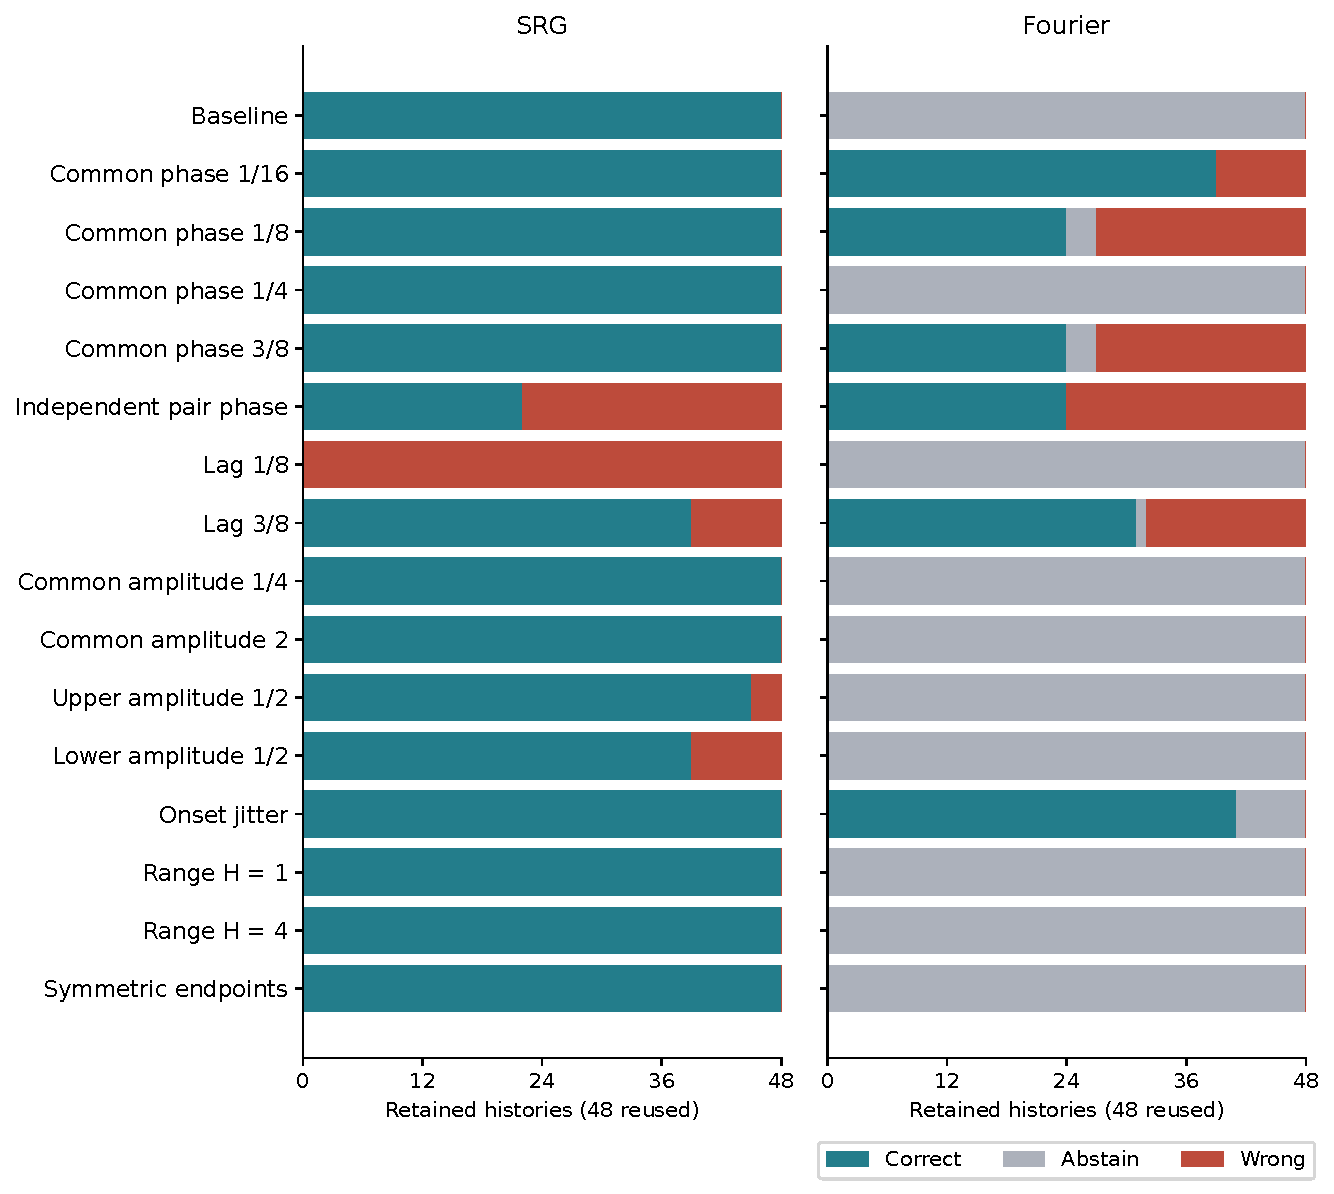
\includegraphics[width=\linewidth]{figures/fig06_controls.pdf}
\caption{All sixteen retained perturbation cells at length 128, with the same 48 order sequences reused in every cell and both bases. Correct, abstaining and covered wrong outcomes are separated. These empirical cells do not establish unrestricted phase, amplitude or history robustness.}
\label{fig:controls}
\end{figure}

\subsection{Projection is a numerical increment, not physical dissipation}
\begin{proposition}[Quadratic account under projection]\label{prop:projection}
For any directional state $x$, event increment $v$ and numerical map $Q$, let $z=x+v$, $x'=Qz$. Then
\begin{equation}\label{eq:projection}
 \E(x')-\E(x)=x\cdot v+\tfrac12\norm v^2
              +\tfrac12\bigl(\norm{Qz}^2-\norm z^2\bigr).
\end{equation}
The mean can be changed independently without affecting the harmonic decision, but remains part of the stored state and this account. In moment coordinates the corresponding metric is $\E(\Tp y)$.
\end{proposition}
\begin{proof}
Add and subtract $\norm{x+v}^2/2$, then expand its difference from $\norm x^2/2$. Coordinatewise quantization updates the mean without mixing it into the four harmonic coordinates; the decision \eqref{eq:storage} contains no mean. This proves decision independence, not permission to omit the mean from storage. Substitution $x=\Tp y$ gives metric matrix $\Tp^{\mathrm T}\Tp/2$ in moment variables.
\end{proof}
The final bracket is an additional numerical projection term. Pure axis clipping toward an interval containing zero cannot increase any absolute coordinate, so its Euclidean contribution is nonpositive; rounding can increase it. Independent Fourier-axis clipping is not Euclidean projection in the $\Tp^{\mathrm T}\Tp$ metric and need not share that argument.

At length 128 the clipped mean is at most $2-\Delta$ instead of 128, replacing the lossless mean account 8192 by approximately two. This is a different state. The projection term is not an implementation of C1 source work, native heat, emitted energy, physical dissipation or a conserved physical quantity.

Diagnostics distinguish overflow of a \emph{rounded code} from a direct unrounded value outside the interval. A small direct residual can round to an allowed boundary and produce no overflow count. CLIP\_ONLY retains the original rounded-trigger diagnostic separately from actual continuous clipping. Traces also record rounding changes, signed and absolute lost increments and projection-account changes. These belong to the evaluator and never enter the decoder.

The single mechanism evaluation took $56.843$ s, with peak working set 111,869,952 bytes and peak pagefile use 127,045,632 bytes. It is not a new cost contest. Its initial precheck failed at Python's integer-string serialization limit; only presentation of enormous rational bounds was changed to compact outward bounds, preserving proof arithmetic and scoring. The accepted record retains that failure, fourteen successful pre-run groups, eight saved-result audit groups and a separate rational eighth-lag certificate. These historical counts are not new manuscript validations.

\section{Consequences and limits}\label{sec:closing}
The completed one-circuit family admits an exact mean-plus-first-harmonic residual after forcing ends. Its five real coordinates are sufficient for that family and its late conditional observation records, not arbitrary shapes, active forcing or the full native state. Duration changes expose this boundary explicitly.

The directional and two-port Fourier forms are invertibly equivalent before nonlinear projection. They contain the same exact information. A single isolated pair yields a valid order feature within a known sub-half-period domain; periodic aliases are part of the feature, while direct timestamps solve the narrower descriptor-order problem without them.

A persistent lossless aggregate has a different meaning from its latest input. The aligned majority identity explains one controlled regime, and an exact state-and-metadata collision rules out universal latest-order decoding there. Quadratic accumulation retains the mean and interference. Idle coefficient persistence incurs no updates and supplies no dynamical stability experiment.

Observation access adds its own restrictions. The full and mirror channels can identify a complex directional pair under the stated calibration; equatorial scalar records cannot. The retained arithmetic-band decoder falsely resolves noisy ties. These limitations coexist with good separated-pair accuracy. A noise-aware receiver would require a separate design, not an editorial correction to the reported result.

The actual software measurements favor timestamps in the narrow events-to-order median and show overlapping timing ranges between coordinate representations. Payload, object headers, shared matrices, calibration and acquisition latency remain charged in their appropriate categories. No asymptotic, hardware, quantum or energy-efficiency advantage follows.

Repeated saturation changes the algorithm. The chronological maps prove a useful incoming-state corner mechanism and sufficient consecutive-label entrance bounds; they also prove an independent Fourier corner abstention and exact same-operator conjugacy. These are restricted numerical facts. Two-write collisions, three-write errors and long-prefix dependence remain. The stronger eighth-lag theorem establishes a uniform \emph{wrong-sign} regime for the fixed decoder under its precise ideal-map assumptions. State label dependence and decoder correctness are distinct even in that regime.

These results support a compact analytic aggregate and a sharply delimited study of nonlinear numerical retention. They do not establish universal latest-write memory, associative capacity, a native circulation claim or a deployable noisy classifier. The geometric motivation remains valuable because it led to explicit questions and discriminating results, including failures.

\subsection*{Authorship and computational assistance}
Hilmir Frímann Halldórsson supplied the geometric and computational motivation and directed the research sequence. OpenAI ChatGPT/GPT and Codex assisted with formalization, source recovery, derivations, software, internal review and manuscript preparation. Internal acceptance of the underlying studies is distinct from external peer review or publication approval of this draft. No affiliation, external proof-audit claim, coauthor consent or license is inferred.

\subsection*{Data and reproducibility}
The accompanying manuscript supplement identifies the unchanged source editions, retained data, static figure scripts and checks of displayed formulas. Its reproduction guide separates document rebuilding and saved-data tabulation from historical experimental programs. Original pilot runs and mechanism results remain retained evidence; they were not rerun to prepare this paper. Complete conditions include failures, abstentions, raw timing repetitions and resource qualifications. The present edition is a local manuscript draft.

\appendix
\section{Rational rounding certificates and proof reproducibility}\label{app:rational}
The map theorems use mathematical integer increments, not a heuristic decimal rounding argument. We restate a finite rational construction from the accepted mechanism source.~\cite{Mechanism} For $q>1$, let
\[
 A_m(q)=\sum_{j=0}^{m-1}\frac{(-1)^j}{(2j+1)q^{2j+1}},\qquad
 R_m(q)=\frac{(-1)^m}{(2m+1)q^{2m+1}}.
\]
The alternating-series remainder puts $\arctan(1/q)$ between $A_m(q)$ and $A_m(q)+R_m(q)$. With $m=36$, the identity
$\pi=16\arctan(1/5)-4\arctan(1/239)$ gives rational endpoints $\pi_-,\pi_+$. For completeness, the tangent double-angle formula gives $\tan(2\arctan(1/5))=5/12$ and $\tan(4\arctan(1/5))=120/119$. Subtracting $\arctan(1/239)$ gives tangent one; the difference is in $(0,\pi/2)$, so it equals $\pi/4$. Thus the stated identity requires no assumed decimal value of $\pi$.

Let
\[
 P_m(x)=\sum_{j=0}^{m}\frac{(-1)^j x^{2j}}{(2j+1)!}.
\]
On the small positive interval around $\pi/32$, alternating terms decrease, hence $P_9(x)\le\sinc x\le P_8(x)$. Also $\sinc$ decreases there: $\sin x-x\cos x=\int_0^x t\sin t\dd t>0$ for $0<x<\pi$. Therefore
\begin{equation}\label{eq:rationalB}
 P_9(\pi_+/32)^2\le B_1\le P_8(\pi_-/32)^2 .
\end{equation}
All bounds are positive, so squaring preserves the inequalities.

For positive rational $v$ and $S=10^{45}$, define
$k=\lfloor\sqrt{\lfloor vS^2\rfloor}\rfloor$ by integer square root. Then
$(k/S)^2\le v<((k+1)/S)^2$, proving a rational square-root enclosure. Apply it to $3/7,4/7,2$. Multiplying the positive $B_1$ and radical intervals gives $c_0,s_0,B_1/4$. For eighth lag, if these bounds are $[c_-,c_+]$, $[s_-,s_+]$, $[\rho_-,\rho_+]$ for $\sqrt2$, positivity gives
\[
 \frac{s_--c_+}{\rho_+}\le e\le\frac{s_+-c_-}{\rho_-},
 \qquad
 \frac{s_-+c_-}{\rho_+}\le f\le\frac{s_++c_+}{\rho_-}.
\]
Divide by the exact positive step and compare with $k\pm1/2$. The accepted rational endpoints, retained in the supplement, lie inside these wider outward rational intervals:
\begin{center}
\begin{tabular}{rrrr}\toprule
$b$ & $c_0/\Delta$ & $s_0/\Delta$ & $B_1/(4\Delta)$\\\midrule
8 & $(10.440850,10.440851)$ & $(12.056055,12.056056)$ & $(15.948661,15.948662)$\\
12 & $(167.053600,167.053601)$ & $(192.896881,192.896882)$ & $(255.178589,255.178590)$\\
16 & $(2672.857601,2672.857602)$ & $(3086.350111,3086.350112)$ & $(4082.857427,4082.857428)$\\\bottomrule
\end{tabular}
\end{center}
At width 12, $18.273959<e/\Delta<18.273960$ and
$254.523426<f/\Delta<254.523427$. Every displayed decimal endpoint is an exact rational with denominator $10^6$. Each interval lies strictly between the half-integer neighbors of its code, proving the rounding choices without a half-tie ambiguity. The narrow source endpoints and their outward serialization are copied unchanged; the manuscript-local checker verifies their containment and consequences rather than replaying the original large suite.

\section{Complete endpoint and measurement tables}\label{app:data}
The tables below use saved records only. In a non-tie set of size $n$, let $C$ be correct decisions, $A$ abstentions and $W$ covered wrong decisions. Coverage is $(C+W)/n$ and covered error is $W/(C+W)$ when the denominator is nonzero. Unconditional correct fraction is $C/n$. Simultaneous truth is reported separately as false resolved signs, rather than being hidden in a non-tie accuracy denominator.

Each operation or perturbation row reuses 48 histories, so neither widths nor cells are independent replications. Full prefix tables and coordinate diagnostics remain in the accompanying complete-condition data. The main text states the theoretical domains; counts alone do not generalize them.
\begin{longtable}{P{65mm}rrr}
\caption{Every operation endpoint at width 12. Each row reuses the same 48 histories; C/A/W means correct/abstain/covered wrong.}\\
\toprule Basis / operation & C/A/W & Coverage & Min $\ell\eta$\\\midrule\endfirsthead
\toprule Basis / operation & C/A/W & Coverage & Min $\ell\eta$\\\midrule\endhead
Fourier / CLIP\_ONLY & 0/48/0 & 0.000 & -0\\
Fourier / FINAL\_CLIP & 0/48/0 & 0.000 & -0\\
Fourier / LOSSLESS & 26/3/19 & 0.938 & -0.316417\\
Fourier / PAIR\_CLIP & 0/48/0 & 0.000 & -0\\
Fourier / ROUND\_CLIP & 0/48/0 & 0.000 & -0\\
Fourier / ROUND\_ONLY & 26/3/19 & 0.938 & -0.316417\\
Fourier / SYMMETRIC\_ENDPOINT & 0/48/0 & 0.000 & -0\\
Fourier\_conjugated / CONJUGATED\_Q & 48/0/0 & 1.000 & 0.0539721\\
SRG / CLIP\_ONLY & 48/0/0 & 1.000 & 0.0539048\\
SRG / FINAL\_CLIP & 0/48/0 & 0.000 & -0\\
SRG / LOSSLESS & 26/3/19 & 0.938 & -0.316417\\
SRG / PAIR\_CLIP & 48/0/0 & 1.000 & 0.012779\\
SRG / ROUND\_CLIP & 48/0/0 & 1.000 & 0.0539721\\
SRG / ROUND\_ONLY & 26/3/19 & 0.938 & -0.316673\\
SRG / SYMMETRIC\_ENDPOINT & 48/0/0 & 1.000 & 0.0539965\\
\bottomrule\end{longtable}

\begin{longtable}{P{66mm}rr}
\caption{All sixteen fixed perturbation cells at length 128, 48 reused histories per basis. Each row changes only its named factor.}\\
\toprule Cell & Directional C/A/W & Fourier C/A/W\\\midrule\endfirsthead
\toprule Cell & Directional C/A/W & Fourier C/A/W\\\midrule\endhead
baseline & 48/0/0 & 0/48/0\\
common\_phase\_1\_16 & 48/0/0 & 39/0/9\\
common\_phase\_1\_8 & 48/0/0 & 24/3/21\\
common\_phase\_1\_4 & 48/0/0 & 0/48/0\\
common\_phase\_3\_8 & 48/0/0 & 24/3/21\\
independent\_pair\_phase & 22/0/26 & 24/0/24\\
lag\_1\_8 & 0/0/48 & 0/48/0\\
lag\_3\_8 & 39/0/9 & 31/1/16\\
common\_amplitude\_1\_4 & 48/0/0 & 0/48/0\\
common\_amplitude\_2 & 48/0/0 & 0/48/0\\
upper\_amplitude\_half & 45/0/3 & 0/48/0\\
lower\_amplitude\_half & 39/0/9 & 0/48/0\\
onset\_jitter & 48/0/0 & 41/7/0\\
range\_H1 & 48/0/0 & 0/48/0\\
range\_H4 & 48/0/0 & 0/48/0\\
symmetric\_endpoints & 48/0/0 & 0/48/0\\
\bottomrule\end{longtable}


\subsection{All noise cells}
Noise levels are absolute standard deviations in the normalized output units, not a universal physical SNR specification. Both coordinate decoders process identical records and agree in decisions. Rank-one refusal is an information limit; a fast unresolved return is not a successful direction estimate.
\begin{longtable}{llrrr}
\caption{All saved noise cells; coordinate decoders agree in decisions. Simultaneous controls number 384 per row; false tie signs are separate from non-tie covered errors.}\\
\toprule Format & Group & $\sigma$ & Quarter C/A/W (768) & False tie signs\\\midrule\endfirsthead
\toprule Format & Group & $\sigma$ & Quarter C/A/W (768) & False tie signs\\\midrule\endhead
f64 & full & 0 & 768/0/0 & 0/384\\
f64 & full & 1e-05 & 768/0/0 & 384/384\\
f64 & full & 0.001 & 768/0/0 & 384/384\\
f64 & full & 0.01 & 762/0/6 & 384/384\\
f64 & full & 0.1 & 490/0/278 & 384/384\\
f64 & mirror & 0 & 768/0/0 & 0/384\\
f64 & mirror & 1e-05 & 768/0/0 & 384/384\\
f64 & mirror & 0.001 & 768/0/0 & 384/384\\
f64 & mirror & 0.01 & 690/0/78 & 384/384\\
f64 & mirror & 0.1 & 419/0/349 & 384/384\\
f64 & null & 0 & 0/768/0 & 0/384\\
f64 & null & 1e-05 & 0/768/0 & 0/384\\
f64 & null & 0.001 & 0/768/0 & 0/384\\
f64 & null & 0.01 & 0/768/0 & 0/384\\
f64 & null & 0.1 & 0/768/0 & 0/384\\
f32 & full & 0 & 768/0/0 & 0/384\\
f32 & full & 1e-05 & 768/0/0 & 373/384\\
f32 & full & 0.001 & 768/0/0 & 384/384\\
f32 & full & 0.01 & 762/0/6 & 384/384\\
f32 & full & 0.1 & 490/0/278 & 384/384\\
f32 & mirror & 0 & 768/0/0 & 0/384\\
f32 & mirror & 1e-05 & 768/0/0 & 379/384\\
f32 & mirror & 0.001 & 768/0/0 & 384/384\\
f32 & mirror & 0.01 & 690/0/78 & 384/384\\
f32 & mirror & 0.1 & 419/0/349 & 384/384\\
f32 & null & 0 & 0/768/0 & 0/384\\
f32 & null & 1e-05 & 0/768/0 & 0/384\\
f32 & null & 0.001 & 0/768/0 & 0/384\\
f32 & null & 0.01 & 0/768/0 & 0/384\\
f32 & null & 0.1 & 0/768/0 & 0/384\\
\bottomrule\end{longtable}


\subsection{All matched timing cells}
The following table uses the corrected single-thread run only. J1 is events-to-order, J2 events-to-record and J3 samples-to-direction. Float32 denotes mixed state/sample precision, with binary64 input clocks and fitting arithmetic as specified in the text. Timestamp code remains binary64 in both J1 lanes. All seven raw repetition totals, batch sizes, warmups, rotated method order, overhead loops and calibration-growth records are retained separately. The measured ranges are descriptive and do not establish confidence intervals or worst-case performance.
\begin{longtable}{P{43mm}lll}
\caption{All 26 corrected timing cells; seven raw repetitions per row. Null timings measure abstention, not identification.}\\
\toprule Job/group & Format & Method & Min/median/max ($\mu$s)\\\midrule\endfirsthead
\toprule Job/group & Format & Method & Min/median/max ($\mu$s)\\\midrule\endhead
J1/events\_to\_order & f64 & SRG & 12.087/17.263/19.651\\
J1/events\_to\_order & f64 & Fourier & 13.582/19.210/19.690\\
J1/events\_to\_order & f64 & Timestamps & 10.154/12.933/14.646\\
J2/full\_one & f64 & SRG & 19.798/40.403/47.275\\
J2/full\_one & f64 & Fourier & 41.910/45.196/54.286\\
J2/all84 & f64 & SRG & 61.100/64.534/70.887\\
J2/all84 & f64 & Fourier & 44.819/67.250/73.219\\
J3/full\_one & f64 & SRG & 13.095/14.532/16.525\\
J3/full\_one & f64 & Fourier & 14.534/16.677/21.288\\
J3/mirror\_scalar & f64 & SRG & 11.853/14.653/17.352\\
J3/mirror\_scalar & f64 & Fourier & 14.920/17.817/20.389\\
J3/null & f64 & SRG & 8.228/10.933/11.377\\
J3/null & f64 & Fourier & 7.570/10.485/11.317\\
J1/events\_to\_order & f32 & SRG & 16.630/18.537/20.992\\
J1/events\_to\_order & f32 & Fourier & 16.922/21.645/24.493\\
J1/events\_to\_order & f32 & Timestamps & 10.133/13.822/14.370\\
J2/full\_one & f32 & SRG & 31.202/48.382/50.854\\
J2/full\_one & f32 & Fourier & 25.757/47.731/62.550\\
J2/all84 & f32 & SRG & 54.476/67.565/74.474\\
J2/all84 & f32 & Fourier & 41.740/67.529/82.734\\
J3/full\_one & f32 & SRG & 13.558/15.590/17.881\\
J3/full\_one & f32 & Fourier & 16.392/18.860/21.737\\
J3/mirror\_scalar & f32 & SRG & 7.202/16.063/17.500\\
J3/mirror\_scalar & f32 & Fourier & 16.700/19.083/20.687\\
J3/null & f32 & SRG & 7.260/10.434/12.124\\
J3/null & f32 & Fourier & 8.929/10.953/12.173\\
\bottomrule\end{longtable}


\begin{thebibliography}{9}
\raggedright
\bibitem{PaperI}
H. F. Halldórsson.
\emph{Paired-Gap Geometry and Toroidal Observation Maps for the Folded Tri-Octagon}.
Paper I, v0.1.1, 2026. Author-published repository edition, commit
\href{https://github.com/pzychozen/trioctagon-physics/commit/88ee0550f851507c159f4443c999b6f3ae39097d}{88ee0550f851507c159f4443c999b6f3ae39097d}.
\bibitem{PaperII}
H. F. Halldórsson.
\emph{Paired Driving and Exterior Identifiability on a Conditional Periodic Carrier}.
Paper II, v0.1, 2026. Author-published repository edition, commit
\href{https://github.com/pzychozen/trioctagon-physics/commit/a208add23e892d9a35b4e6a764a2cd1bff60ce56}{a208add23e892d9a35b4e6a764a2cd1bff60ce56}.
\bibitem{Pilot}
H. F. Halldórsson research programme, with Codex computational assistance.
\emph{SRG-Computational-Pilot-09: standalone compact-state pilot}.
18 October 2026. Unpublished research report, prototype contract, frozen benchmark specification, completed-event source implementation, corrected saved results and two-run lineage. Source copies in the manuscript supplement.
\bibitem{Mechanism}
H. F. Halldórsson research programme, with Codex computational assistance.
\emph{SRG-Clipping-Mechanism-10: saturation explains the subset; fixed controls delimit it}.
18 October 2026. Unpublished report, mechanism theorems T1--T7 and counterexamples C1--C4, complete condition tables, rational certificates, frozen plan and saved outcomes. Source copies in the manuscript supplement.
\bibitem{Review09}
OpenAI GPT.
\emph{SRG-Computational-Pilot-09: mathematical/software review}.
18 October 2026. Internal review and acceptance record; includes the aligned-majority deduction and Fourier endpoint/abstention clarification. Not external peer review.
\bibitem{Review10}
OpenAI GPT.
\emph{SRG-Clipping-Mechanism-10: mathematical/software review}.
18 October 2026. Internal review and acceptance record; includes the all-grid failure proof review and additive source-locator clarification. Not external peer review.
\end{thebibliography}

\end{document}
